\chapter{Results}
\label{ch:results}

This chapter presents the results of the project to address our research question. 
\begin{mainbox}{} 
      \textit{How can design theories and principles of information visualization, combined with an iterative development process, be applied to improve the usability and functionality of a website monitoring dashboard? }
\end{mainbox}
The results comprise of qualitative and quantitative results from user testing, as well all requirements that were elicited and implemented in accordance with the process outlined in \autoref{sec:req_gathering}. The chapter aims to show the how the monitoring dashboard evolved throughout the iterative development process.

\section{Requirements Prior to User Testing}
Requirement gathering occurred in four stages as described in \autoref{sec:req_gathering}. The first stage involved analysing the assignment brief provided by Headspin, and are shown in \autoref{tab:non_functional_reqs_brief-res} and \autoref{tab:non_functional_reqs_brief-res}


\begin{table}[H]
\centering
\caption{Functional Requirements from Brief}
\label{tab:functional_reqs_brief-res}
\begin{tabular}{| l  |p{0.6\textwidth}  |l |} 
\hline
\textbf{Req ID} & \textbf{Requirement Title} & \textbf{Priority} \\
\hline
F.1 & User can add, edit, and delete monitored websites via the user interface.& High \\ \hline 
F.2 & User can set custom check interval per site.& High \\ \hline 
F.3 & Display HTTP status, response time, and uptime history for each website.& High \\ \hline 
F.4 & Verify that a site is actually up (beyond HTTP status).& High \\ \hline 
F.5 & Trigger alerts and notifications via e-mail or sms.& Medium \\ \hline

\hline
\end{tabular}
\end{table}

\begin{table}[H]
    \centering
    \caption{Non-Functional Requirements from Brief}
    \label{tab:non_functional_reqs_brief-res}
    \begin{tabular}{| l  |p{0.6\textwidth}  |l |} 
        \hline
        \textbf{Req ID} & \textbf{Requirement Description} & \textbf{Priority} \\
        \hline
        NF.1 & The system must support monitoring of multiple sites without significant delay.& High \\ \hline 
        NF.2 & Website status changes must be easy to interpret at a glance.& High \\ \hline 
        NF.3 & Interface should be user-friendly and intuitive.& High \\ \hline 
        NF.4 & Code base must be maintainable and well-documented.& Medium \\ \hline
    \end{tabular}
\end{table}

\autoref{tab:stakeholder_functional_res} and \autoref{tab:stakeholder_nonfunc_res} show the results the second stage of requirement gathering, after a clarification meeting was held with Headspin. These requirements were used to create the prototype used in user test 1.
\begin{table}[H]
\centering
\caption{Functional requirements (after stakeholder meeting)}
\label{tab:stakeholder_functional_res}
\begin{tabular}{| l  |p{0.6\textwidth}  |l |} 
\hline
\textbf{ID} & \textbf{Requirement Description}& \textbf{Priority} \\ \hline
F.1 & User can add, edit and delete monitored websites via the user interface.& High \\ \hline
F.2 & User can set custom check interval per site.& High \\ \hline
F.3 & Display HTTP status, response time, and uptime history for each website.& High \\ \hline
F.4 & Verify that a site is actually up (beyond HTTP 200). & High \\ \hline 
F.5 & Trigger alerts and notifications via e-mail or sms.&Medium \\ \hline
F.6 & Implement user authentication with personalized dashboards.& Medium\\ \hline
F.7 & Add functionality for filtering and sorting of websites.& Medium \\ \hline
\end{tabular}
\caption{Functional requirements after stakeholder meeting}
\label{tab:functional_req_stakeholder}
\end{table}

\begin{table}[H]
\centering
\begin{tabular}{| l  |p{0.6\textwidth}  |l |} 
\hline
\textbf{ID} & \textbf{Requirement wording (unchanged)} & \textbf{Priority} \\ \hline
NF.1 & Support monitoring of 50+ sites without noticeable delay.& High \\ \hline
NF.2 & Website status changes must be easy to interpret at a glance. & High \\ \hline
NF.3 & Interface must be user‑friendly and intuitive. & High \\ \hline
NF.4 & Code base should be maintainable and documented. & Medium \\ \hline
\end{tabular}
\caption{Non‑functional requirements after stakeholder meeting}
\label{tab:stakeholder_nonfunc_res}
\end{table}

These requirements were further refined, expanded on, and implemented as described in \autoref{sec:user_test_results}



\section{User Interfaces Evaluated in User Testing}
\label{sec:artefact_snapshot}

This section describes the two versions of the monitoring dashboard that were used to gather feedback in user test 1 and 2. \autoref{fig:dashboards_comparison} shows the prototype dashboard compared to the MVP, and  \autoref{fig:website_details_mvp} Illustrates the details page for each website that was also part of user test 2.


\begin{figure}[H]
    \centering
    \makebox[\textwidth][c]{%
        \begin{minipage}{1.2\textwidth}
            \centering
            \begin{subfigure}{0.49\textwidth}
                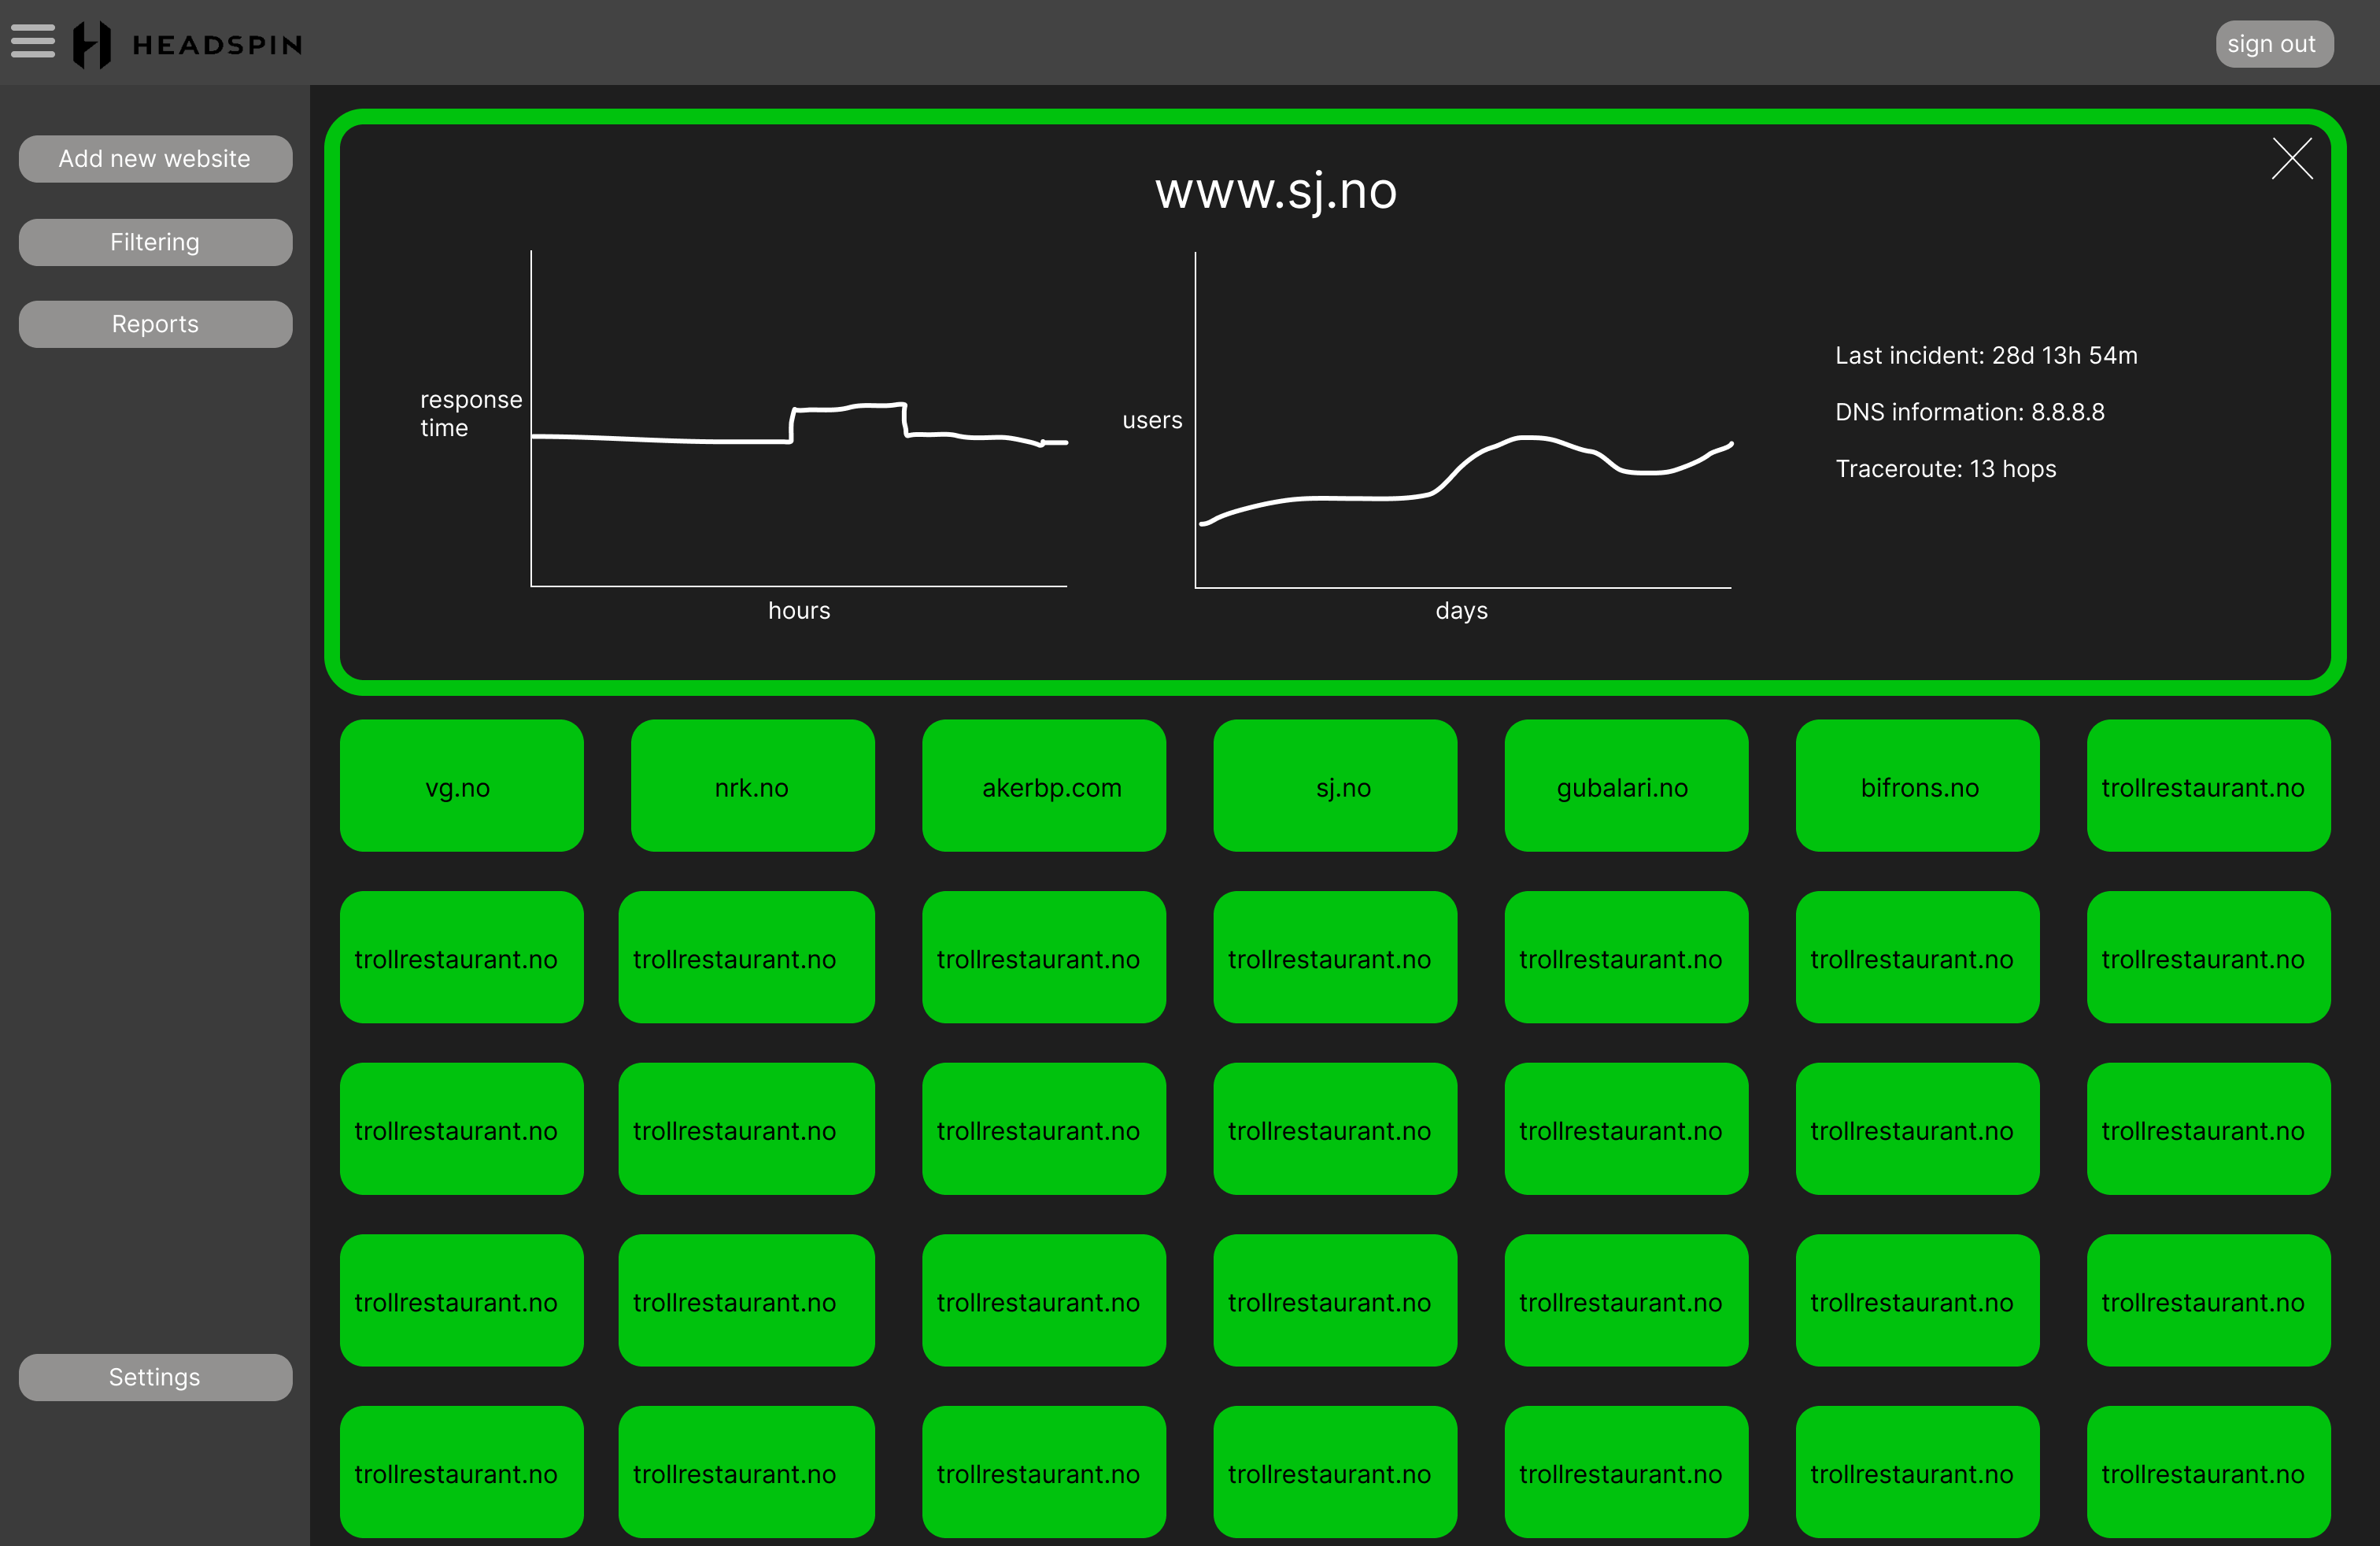
\includegraphics[width=\linewidth]{figures/prototype/prototype_dashboard.png}
                \caption{Prototype dashboard (User Test 1)}
                \label{fig:prototype_dashboard}
            \end{subfigure}
            \hfill
            \begin{subfigure}{0.49\textwidth}
                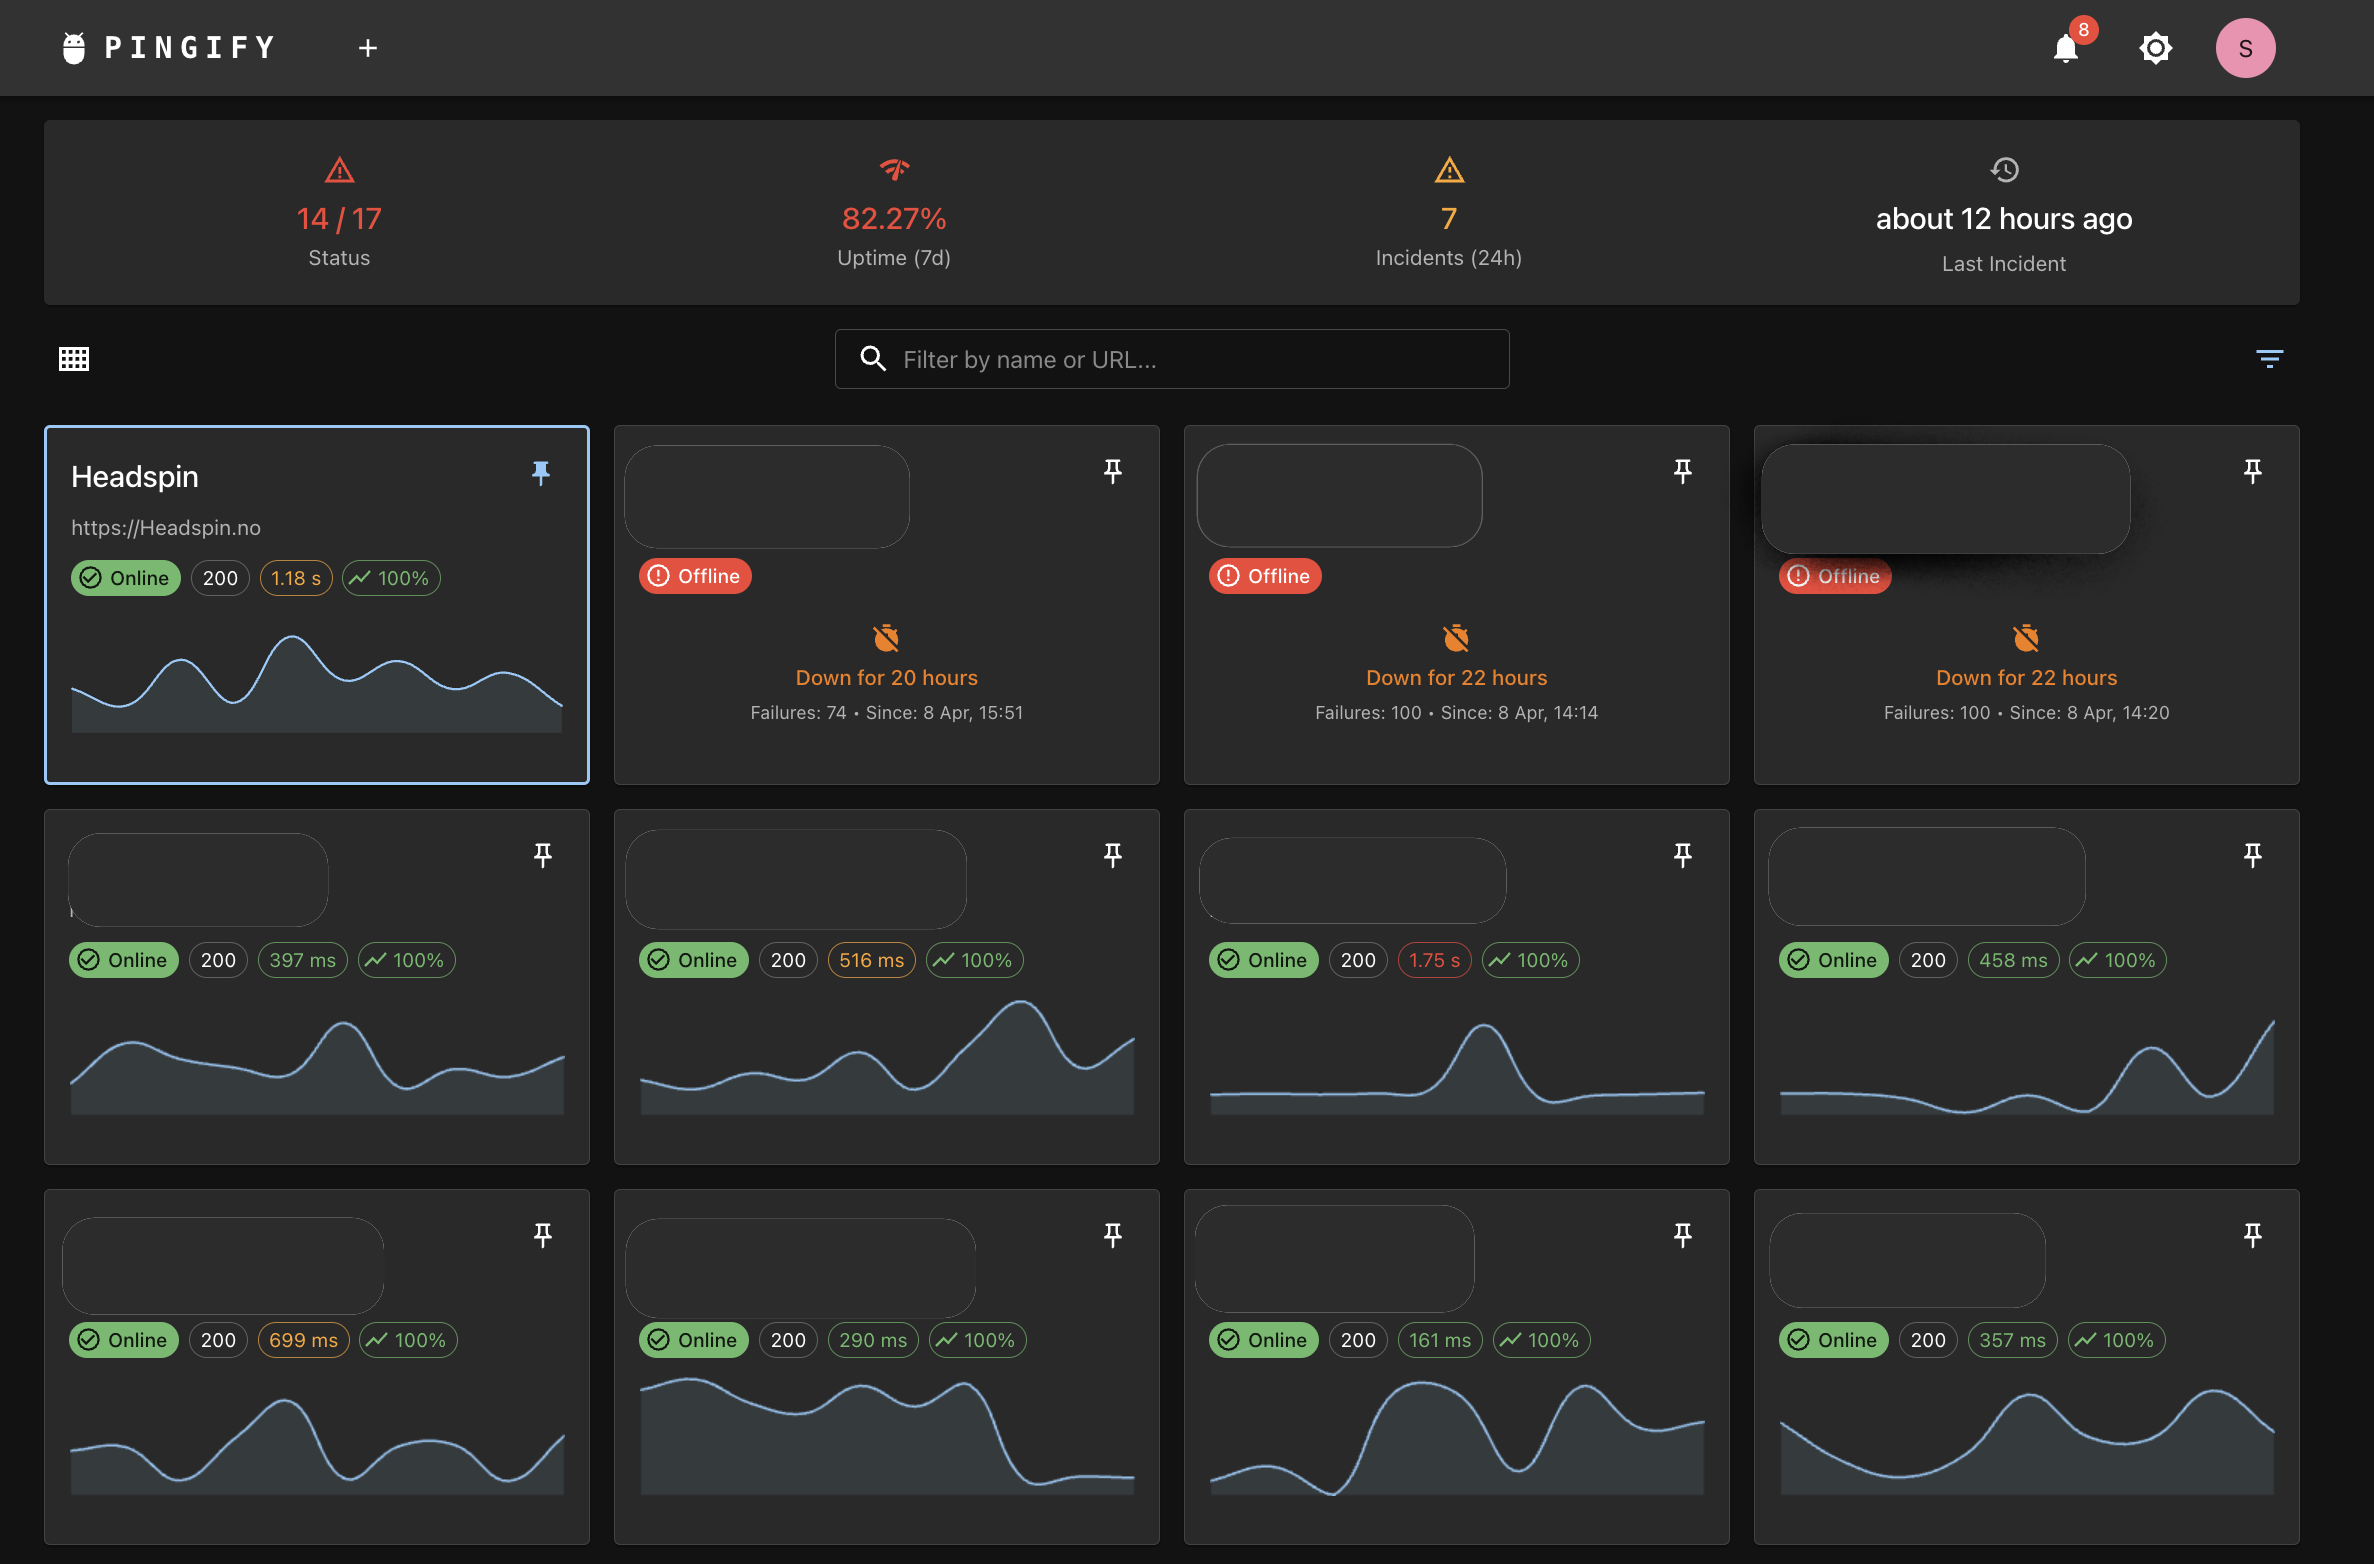
\includegraphics[width=\linewidth]{figures/MVP-dashboard/MVP-dash.png}
                \caption{MVP dashboard (User Test 2)}
                \label{fig:mvp_dashboard}
            \end{subfigure}
        \end{minipage}
    }
    \caption{Dashboards evaluated in the two usability studies.}
    \label{fig:dashboards_comparison}
\end{figure}

\paragraph{Prototype}
The prototype consists of a grid of green cards, where each card shows the status (up/down) of a website based on the colour of the card. When clicked, a window appears at the top of the dashboard, showing details and graphs for that specific website. The prototype has a navigation bar at the top of the page, as well a side bar that can be opened and closed.

\paragraph{MVP}
The MVP also uses a grid with clickable cards for each website on the dashboard. However, clicking on a card in the MVP takes the user to a new page showing details for the website. Where the detailed view was in the prototype, header showing general stats of all website on the dashboard was placed.






\section{Results From User Testing}
\label{sec:user_test_results}
This section addresses findings related to our first research question by presenting both qualitative and quantitative results related to the usability of the dashboard application. It also describes how user feedback directly influenced the design of the dashboard throughout the iterative development process, that is explained further in \autoref{ch:methodology}

\subsection{Qualitative results}
Qualitative results were collected through scenario-based user tests, where participants interacted with both the prototype and \acrshort{mvp} while performing realistic tasks for a website monitoring application. Participants were asked to think aloud, which helped us gain deep insights into their experiences, frustrations, and suggestions for improvement. Key findings from these tests are organized below.

Qualitative results were collected through user test 1 and

\subsubsection{Feedback from Prototype (User Test 1)}  
All participants found the website cards too sparse in information. Participant 1 (P1) requested additional data, such as response time in milliseconds and uptime percentages over different time spans (day, month, year), to be shown directly on the cards (Requirement F.8). Participant 3 (P3) found the interface clear at first glance, but also reflected that the cards showed too little information. 

P1 also wanted a display for general stats from all websites on the dashboard (Requirement F.9).  Participant 2 (P2) found the interface to be incomplete without additional information presented on the dashboard. Two participants criticised the colour palette of the dashboard. P1 noted that everything appeared too green and lacked visual distinction, while P2 found the dashboard very green and somewhat cluttered as a first reaction (Requirement NF.5).

P3 proposed the addition of a featured section or a pin function to keep important websites visible at all times, which would support their daily workflow (Requirement F.10). 

Another issue all the participants agreed on was the inclusion of the sidebar, a hamburger menu with submenus for adding new websites, filtering options, reporting functionality, and settings. P1 described this as unnecessary and recommended moving the filtering options central to the dashboard. P3 had similar feedback and included a preference for using the side bar for the placement of these features, and replacing the descriptive text with the use of iconography (Requirement NF.3). P2 showed hesitation when asked to add a new website, and was unsure of where to find this action.



\begin{table}[H]
    \centering
    \begin{tabular}{|c|p{0.72\linewidth}|c|} \hline
    \textbf{ID} & \textbf{Requirement Description} & \textbf{Priority} \\ \hline
         F.8 &  Implement per-website overview of historical data.& High\\ \hline 
         F.9 &  Display general statistics of all monitored websites & High\\ \hline 
         F.10 & Let users pin websites to the top of the dashboard.&Medium\\\hline
         NF.5 &  Dashboard cards should be easy to understand and not overwhelm the user.& High\\ \hline
    \end{tabular}
    \caption{Additional Functional and Non-Functional requirements from user test 1}
    \label{tab:f_req_usertest_1}
\end{table}



\subsubsection{Changes implemented in MVP}  
Addressing requirements NF.2, stating that website status must be easy to interpret at a glance, the cards were redesigned to include indicators for website status, last HTTP status code, response time in ms, and uptime percentage for the last 24 hours. A graph showing response time for each website the last 24 hours was also added to each card. Before user test 2, the colour palette was revamped to address requirement NF.5. The background colour of the dashboard cards was changed to grey, no longer showing website status by changing the background colour of the cards. Instead, website status was displayed by changing the colour of the indicators introduced to address NF.2 between green, orange and red based on if the website is up, responding slowly, or down.


\begin{figure}[H]
    \centering
    \makebox[\textwidth][c]{%
        \begin{minipage}{1.2\textwidth}
            \centering
            \begin{subfigure}{0.49\textwidth}
                
\includegraphics[width=\linewidth]{figures/prototype/prototype_websitecard.png}
                \caption{Prototype website card}
                \label{fig:prototype_dashboard}
            \end{subfigure}
            \hfill
            \begin{subfigure}{0.40\textwidth}
                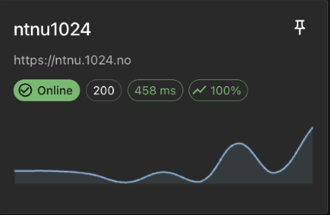
\includegraphics[width=\linewidth]{figures/MVP-dashboard/mvp-card.png}
                \caption{MVP website card}
                \label{fig:mvp_dashboard}
            \end{subfigure}
        \end{minipage}
    }
    \caption{Comparison of website card from prototype to MVP}
    \label{fig:dashboards_comparison}
\end{figure}



A new details page was introduced (Figure~\ref{fig:website_details_mvp}) to address requirement F.8 without cluttering the dashboard. The user navigates to this page by clicking on a website card in the dashboard. This page offers historical data on response time and uptime statistics, in the form of graphs and a list of previous checks. Historical data was introduced on a separate page, to avoid overloading the user with too much information on the main dashboard.


\begin{figure}[H]
  \centering
  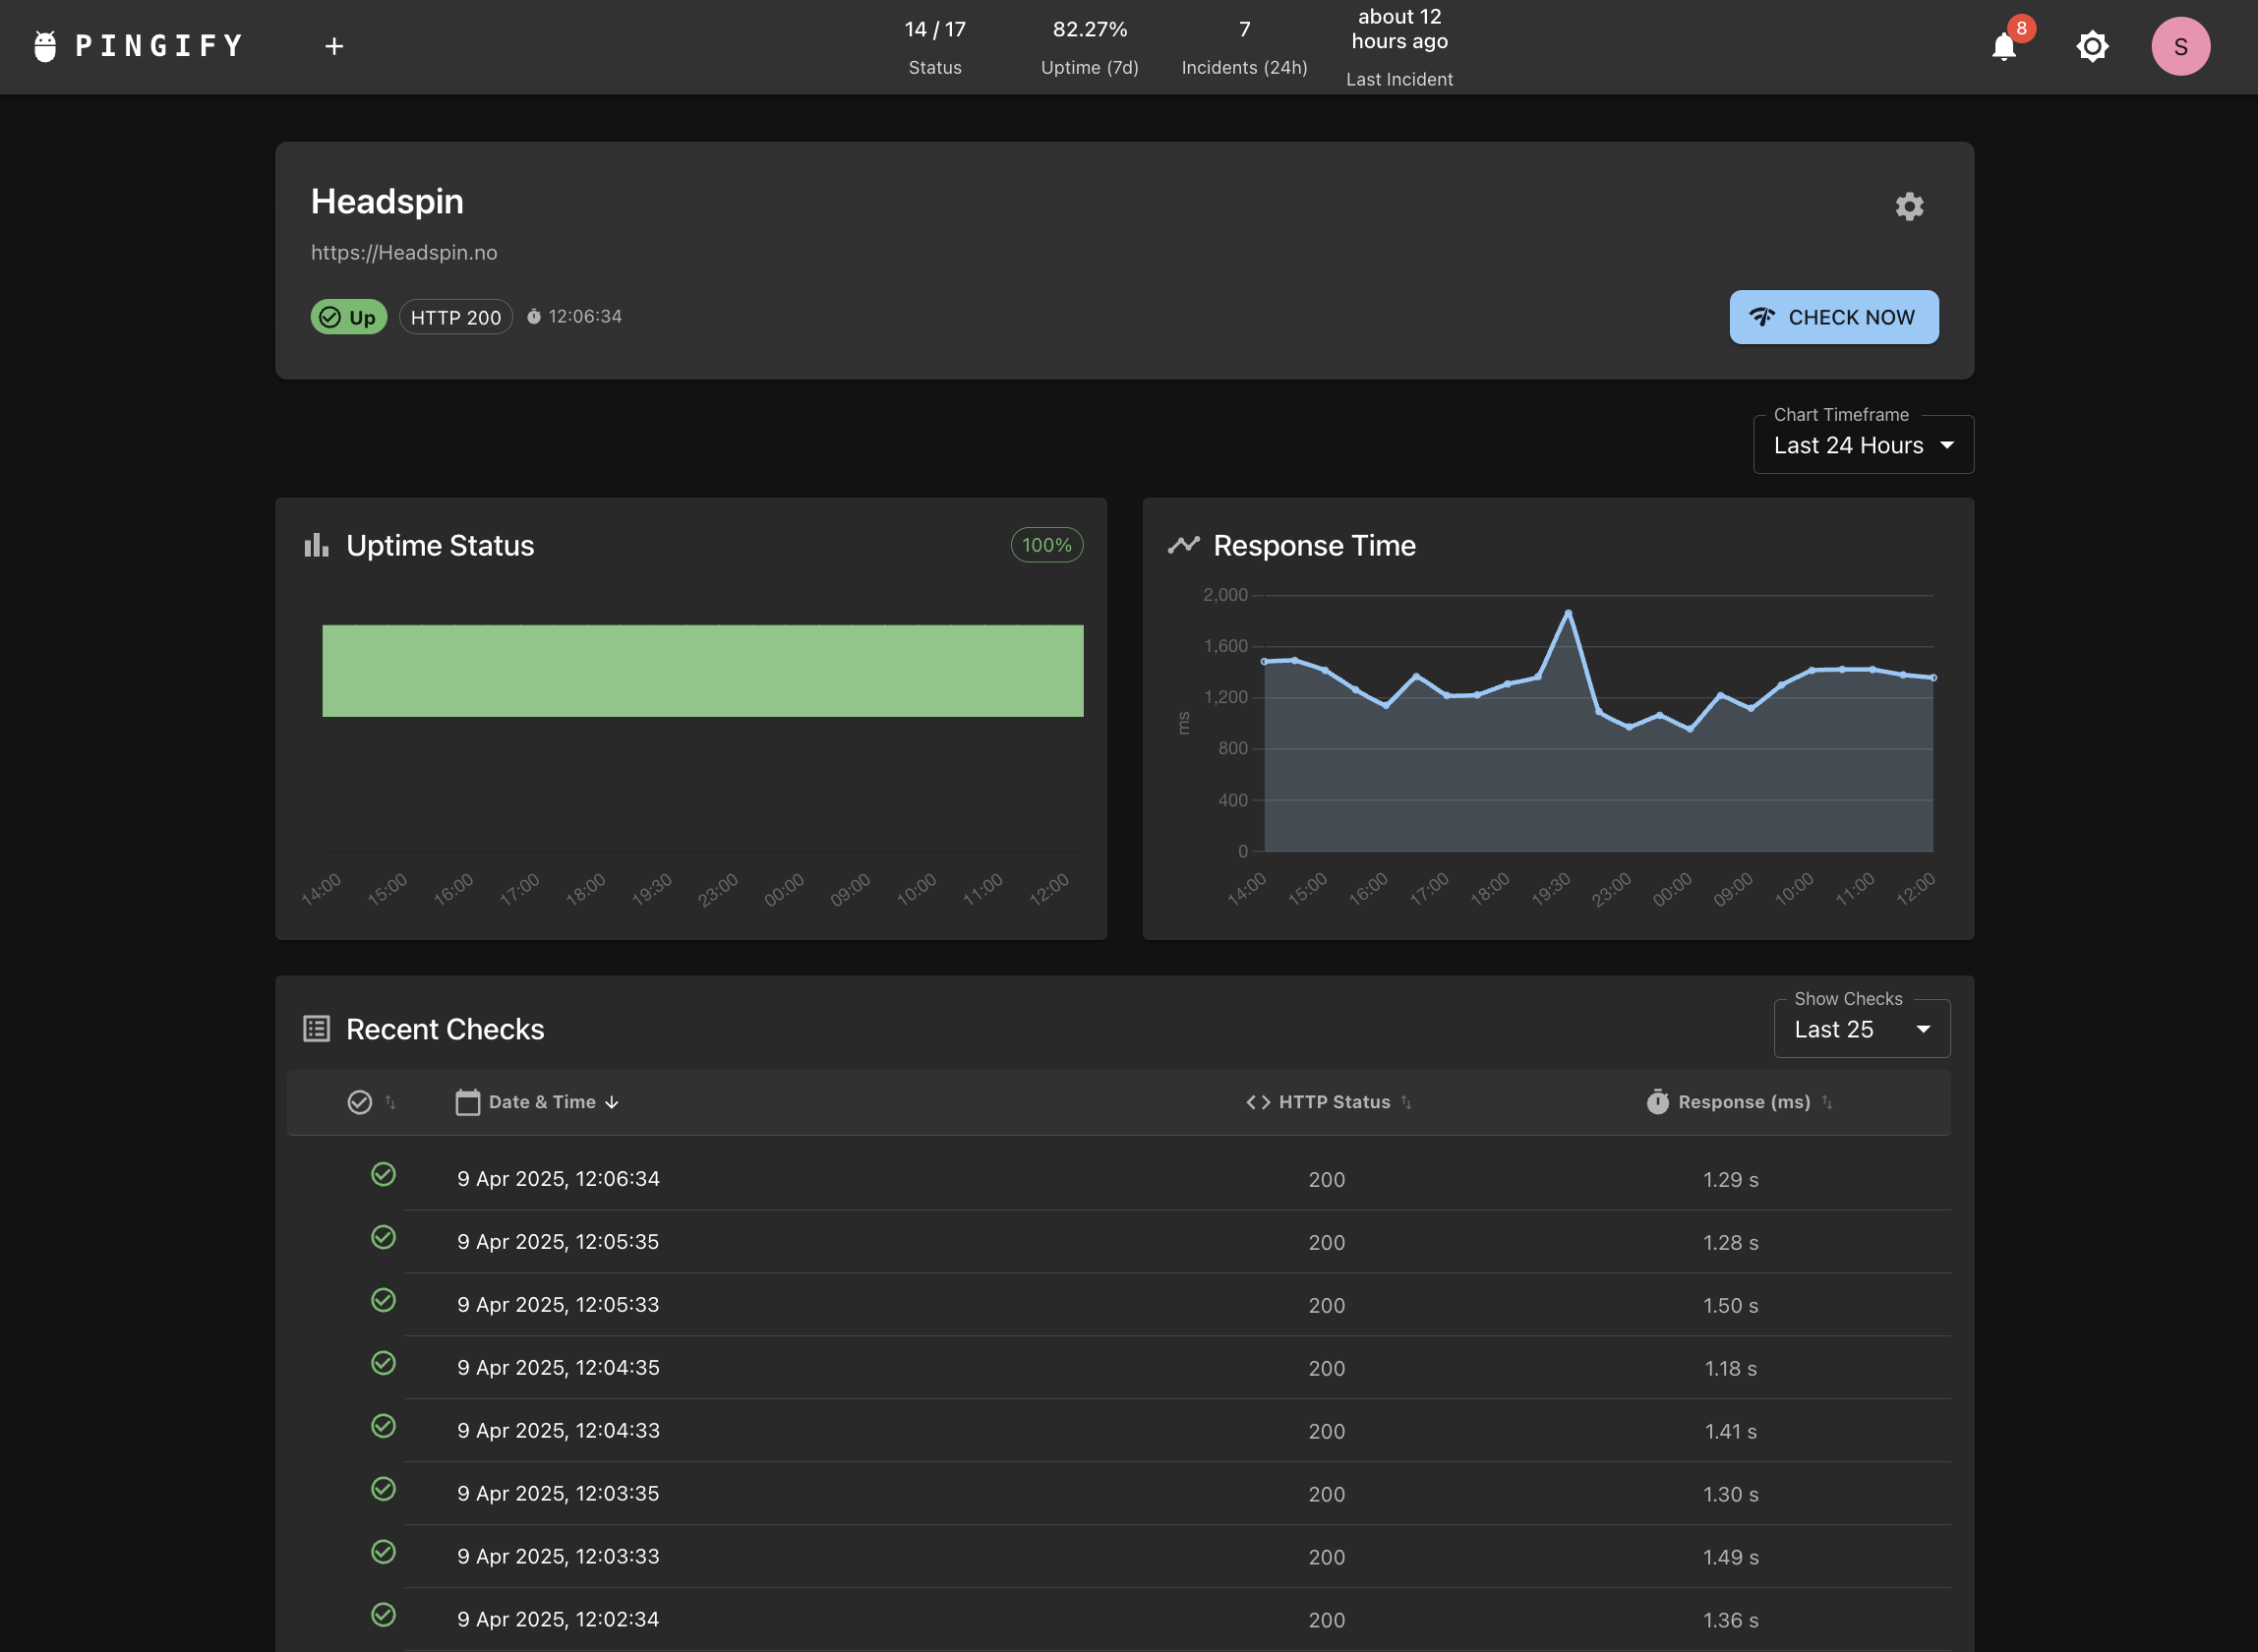
\includegraphics[width=\textwidth]{figures/MVP-dashboard/MVP-websitedetails.png}
  \caption{Website details page in the MVP, showing historical uptime and response time data.}
  \label{fig:website_details_mvp}
\end{figure}
 

Furthermore, the sidebar was completely removed in an attempt to address requirement NF.3, to make the interface more intuitive. The functionality held within was placed elsewhere. For instance the button to add new websites was situated in the navigation bar using a large icon as suggested by P3. This was also where we introduced the alert indicator.  A toggle function for the dark mode/light mode was also situated besides the alert indicator. As well as the new profile icon, which was created as a drawer-menu, opening on click and showing the submenus: profile and logout. The navigation bar also displays status of all monitored websites when the user is not on the main dashboard page. Filtering and sort controls, that were present in the sidebar, were moved to the dashboard itself, keeping it central and close to the objects being filtered and sorted.

\begin{figure}[H]
    \centering
    
\includegraphics[width=1\linewidth]{figures/MVP-dashboard/navbar-mvp.png}
    \caption{Navbar on main dashboard page}
    \label{fig:mvp_navbar}
\end{figure}


\begin{figure}[H]
    \centering
    
\includegraphics[width=1\linewidth]{figures/MVP-dashboard/navbar-mvp-status.png}
    \caption{Navbar showing general status of dashboard when user is not on main dashboard page}
    \label{fig:mvp_navbar_status}
\end{figure}


To address requirement F.9, a banner was introduced to provide an overview of general statistics for all monitored websites. This banner displays key information such as the total number of websites currently up or down, the combined uptime across all sites, the number of incidents in the last 24 hours, and when the last incident occurred. The banner was positioned above the website cards, with the newly implemented "focus mode", along with the search bar and filtering functionality of website cards. 


\begin{figure}
    \centering
    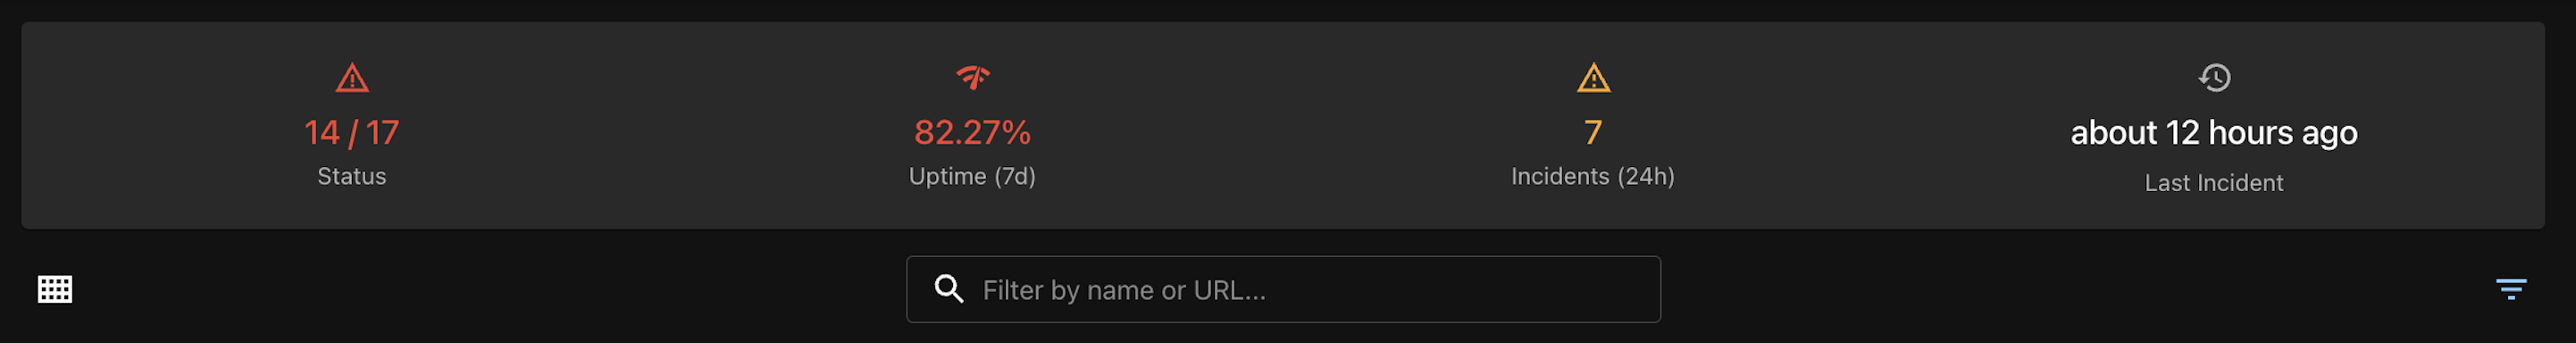
\includegraphics[width=0.8\linewidth]{figures/MVP-dashboard/MVP-statusbanner.png}
    \caption{Status banner with "focus mode", searchbar and filter-button}
    \label{fig:mvp_pinned_card}
\end{figure}


User authentication features were implemented to support user login, registration, and personalized dashboards, responding to requirement F6. This functionality allows multiple users to manage distinct sets of websites within the system. Figure~\ref{fig:login_page} displays how users log in to use the dashboard. When logged in there are certain features which are tracked per-user.

\begin{figure}
    \centering
    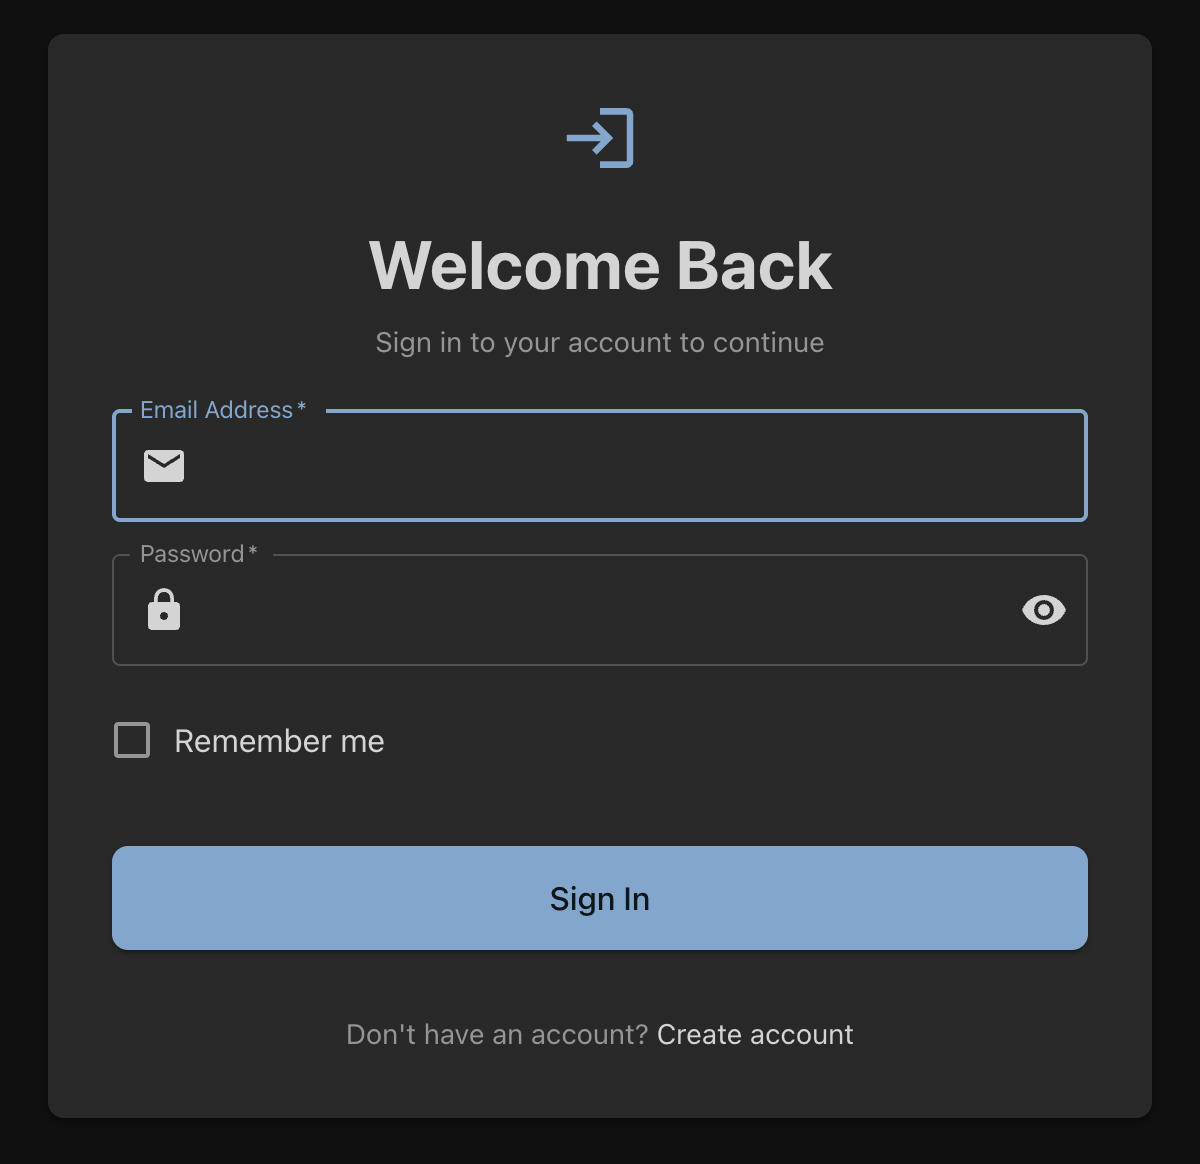
\includegraphics[width=0.75\linewidth]{figures/final_application/final_loginpage.png}
    \caption{Login Page}
    \label{fig:login_page}
\end{figure}


One of these features is pinning. This adheres to requirements F.10 and F.6 and allows users to mark specific websites as important. Pinning a website card automatically moves it to the top of the dashboard, as seen in Figure~\ref{fig:mvp_pinned_card} (also seen in Figure~\ref{fig:mvp_dashboard}).

\begin{figure}
    \centering
    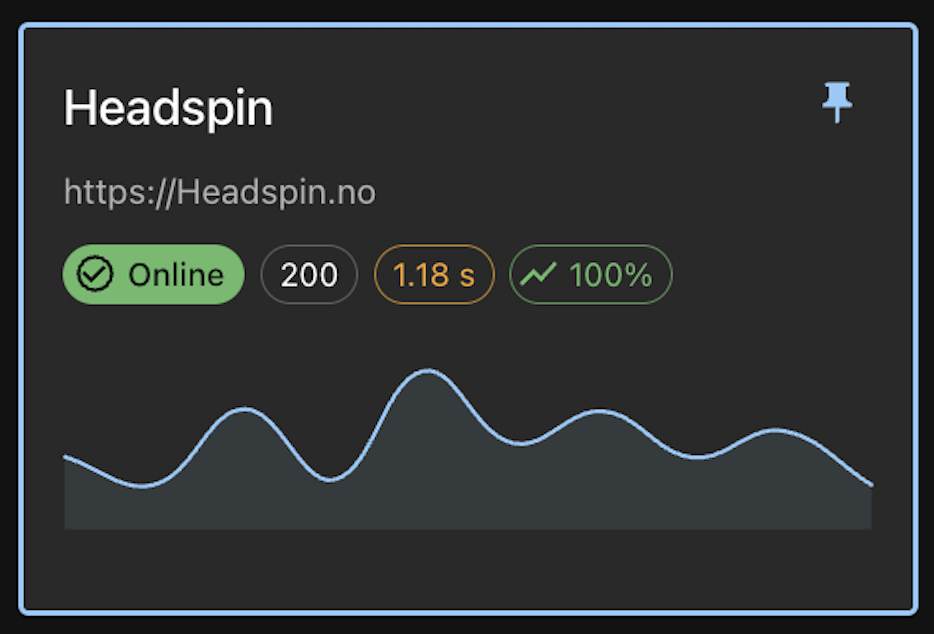
\includegraphics[width=0.5\linewidth]{figures/MVP-dashboard/MVP-pinned-card.png}
    \caption{Pinned Website Card}
    \label{fig:mvp_pinned_card}
\end{figure}


The system's monitoring logic was implemented using \texttt\gls{{axios}} for HTTP requests and the \texttt\gls{{cron}} module to trigger status checks at user-defined intervals, directly addressing F.2. To mitigate false positives, failures were verified by retrying the check after 60 seconds. Two consecutive failures resulted in the generation of an incident log and an alert. Users were provided with the functionality to define thresholds for acceptable response times, and alerts were dispatched only when these defined constraints were violated. Clicking on the alert icon in the navbar opens a list triggered incidents, as illustrated in Figure~\ref{fig:alertlist}

\begin{figure}
    \centering
    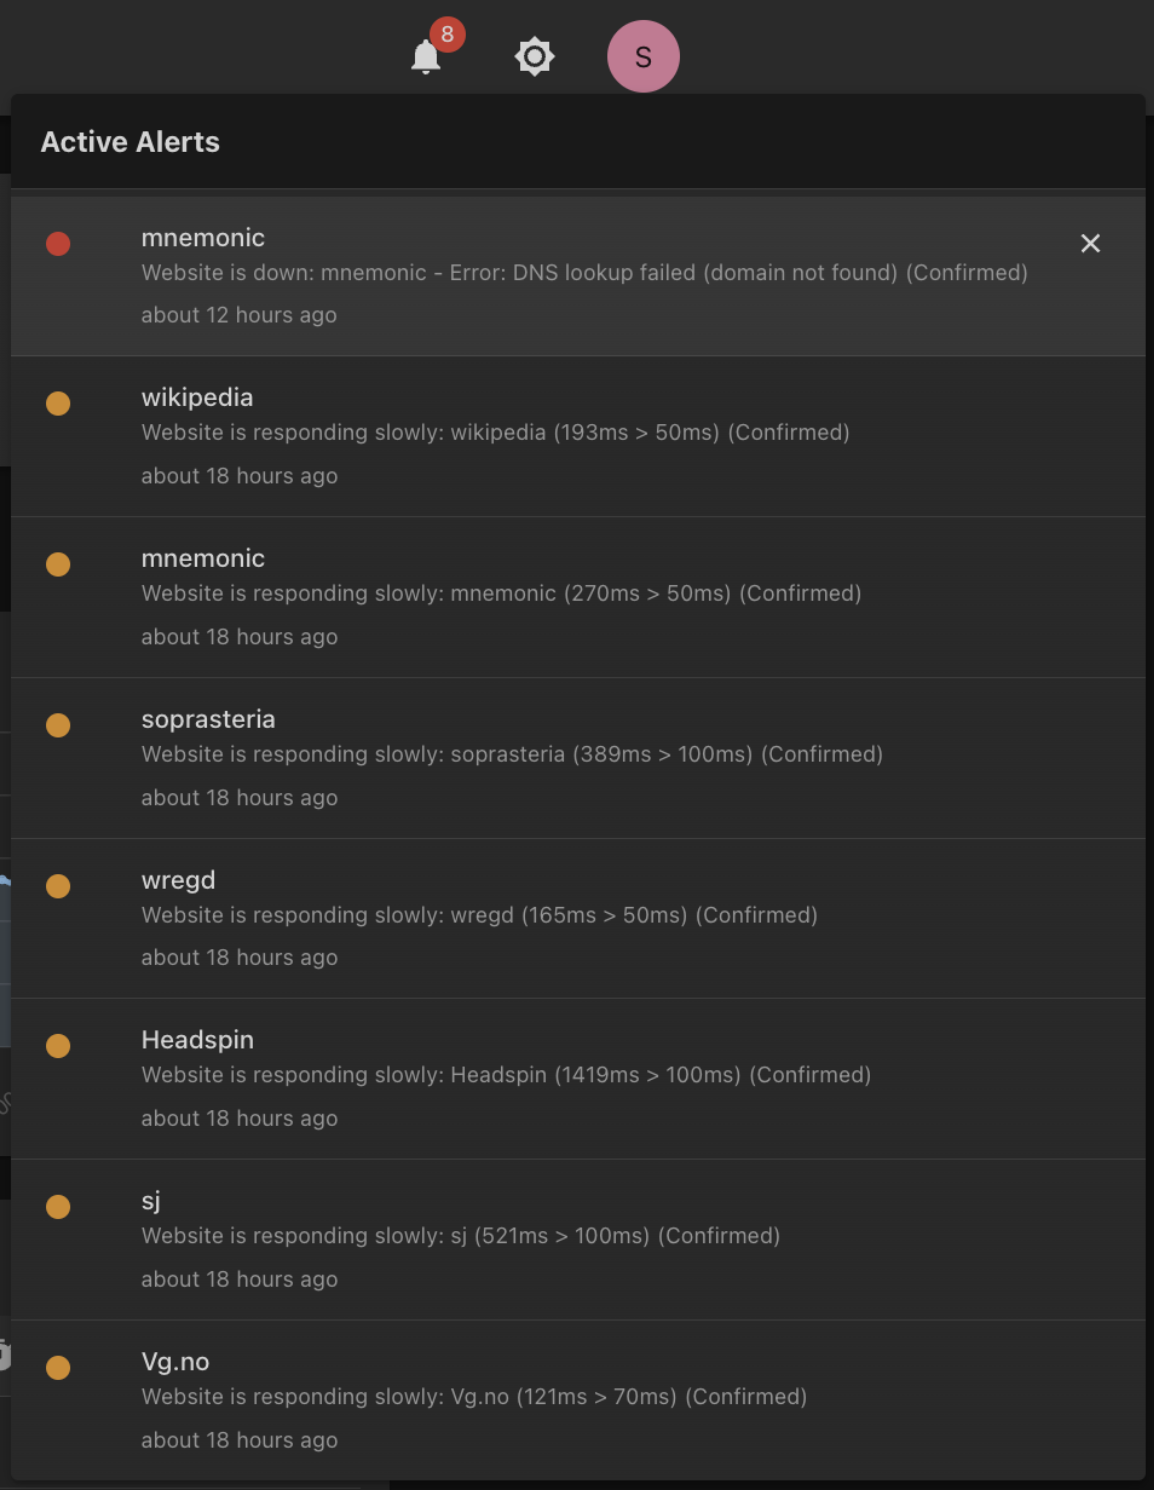
\includegraphics[width=0.65\linewidth]{figures/MVP-dashboard/MVP-only_alertlist.png}
    \caption{List with example alerts}
    \label{fig:alertlist}
\end{figure}

As seen in Figure~\ref{fig:mvpaddwebsite}, adding a new website enables users could configure custom check intervals, in accordance to F.2 and had the options  to enable alerts. Alert settings included defining a response time threshold and specifying a notification email address, fulfilling requirement F.5. 

\begin{figure}
    \centering
    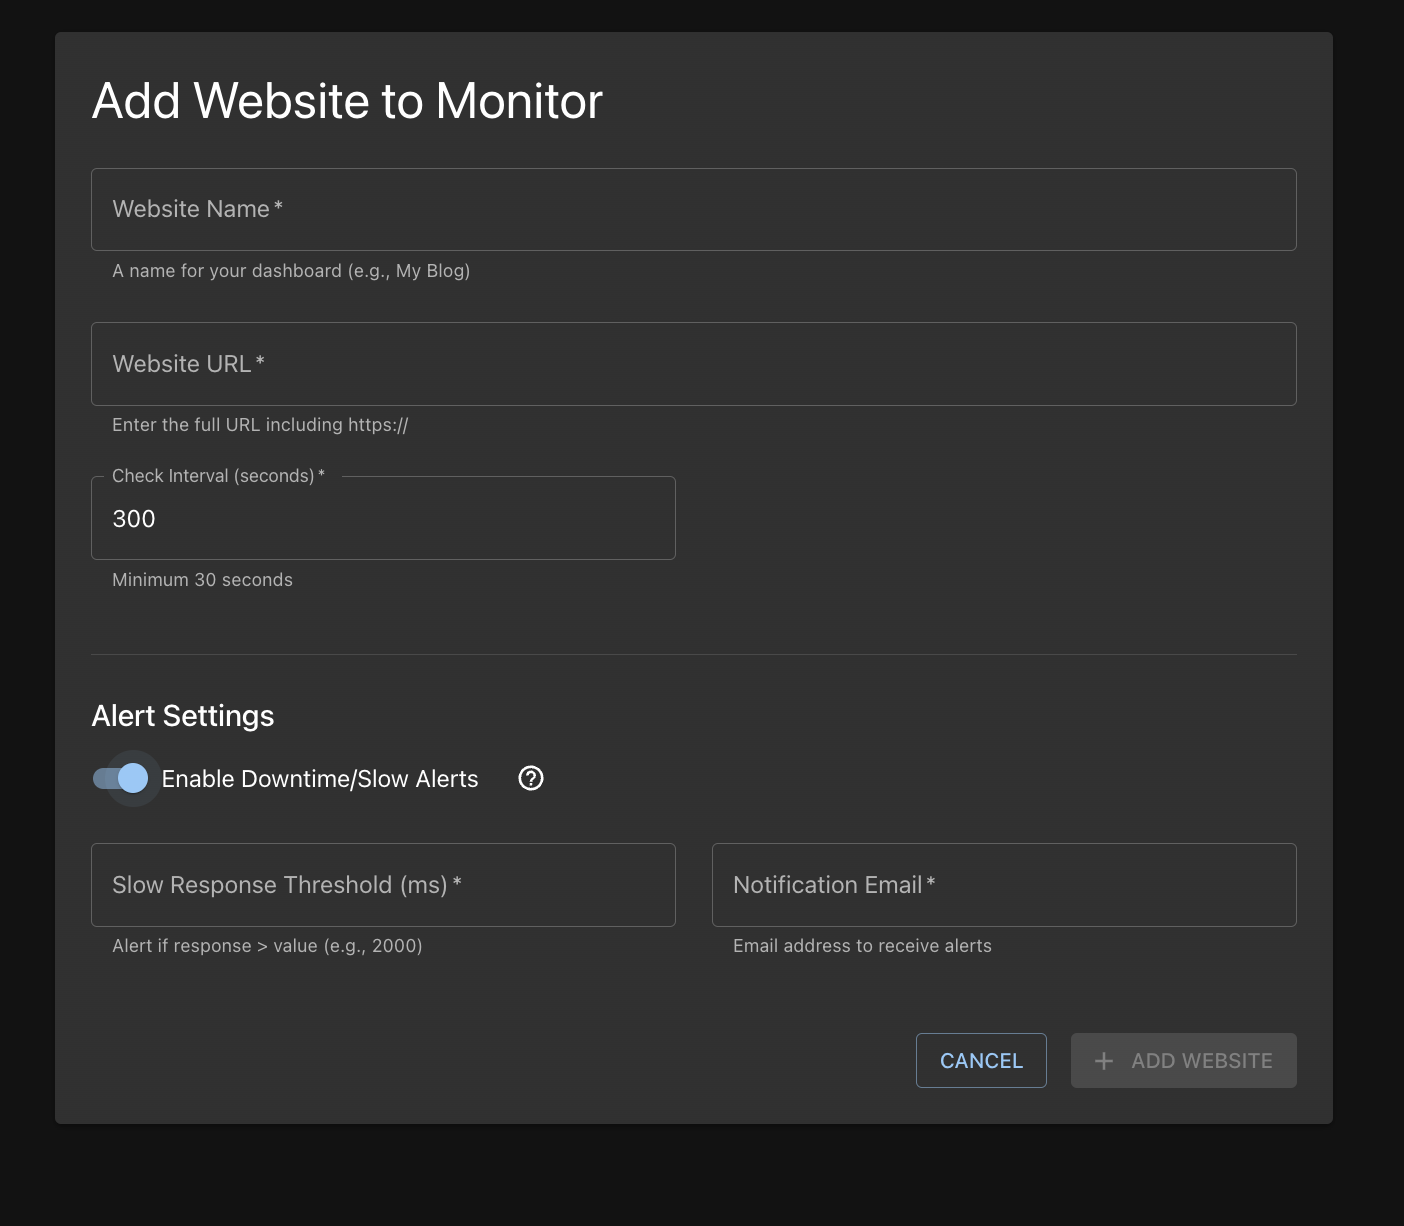
\includegraphics[width=0.6\linewidth]{figures/MVP-dashboard/MVP-addwebsite.png}
    \caption{Options when adding a new website}
    \label{fig:mvpaddwebsite}
\end{figure}



\subsubsection{Feedback from MVP (User Test 2)}  
No participants had any objections to the presentation of the new dashboard cards with the updated status indicators, and changed background colours. However, some new usability issues emerged. All three participants raised confusion about the values represented in the response time graphs on the dashboard cards. P1 commented that the graph lacked a title, legend, and time axis, making it difficult to interpret, Requirement F.11.

P1 also noted that the downtime graph in the Website Details page should be clickable to navigate to a view where the user can see the correlating incident. P2 also suggested that the graph needed clearer colour coding and scaling to represent issue severity.  In addition to verbal feedback, P2 attempted to click on the downtime graph legend, expecting interactivity, indicating a mismatch between user expectations and actual functionality, supporting P1's statement. P1 noted there was a lack of details and a general overview of incidents, Requirement F.12.


Most of the issues regarding navigation were resolved after user test 1, with the addition of the new navigation bar, however two new issues regarding navigation were raised in user test 2. P2 still expressed the need for a more intuitive and central way to add new websites, and P3 spent much time figuring out how to return to the dashboard from the Website Details page, noting the absence of a visible "go back" button. Both address a lack intuitivity of the layout, requirement NF.3. 

We also received feedback from P1, regarding the new status banner, which stated that it took up to much vertical space on the dashboard, that could be used to fit more website cards instead, addressing the already existing requirement NF.2, with system status not being displayed clearly. 



%requireemnts direkte fra MVP user test 2
\begin{table}
    \centering
    \begin{tabular}{|c|p{0.72\linewidth}|c|} \hline
    \textbf{ID} & \textbf{Requirement Description} & \textbf{Priority} \\ \hline
         F.11&  Graphs on cards needs title, legend, and time axis& Medium\\ \hline 
         F.12&  Incident tracking system with incident list& High\\\hline
    \end{tabular}
    \caption{Additional Functional and Non-Functional requirements from user test 2}
    \label{tab:f_req_usertest_2}
\end{table}

\paragraph{Addressing User Test 2 Feedback}

An incident log was introduced to improve contextual understanding of recurring website issues. This feature, developed in response to the new requirement F.12, established after User Test 2 feedback. The incident log enables users to track, review, and visualize incidents based on consecutive monitoring failures. The incidents are accessible from both the main dashboard and the Website Details view, helping users understand service disruptions over time (see Figure~\ref{fig:incident_list}).so

\begin{figure}[H]
\centering
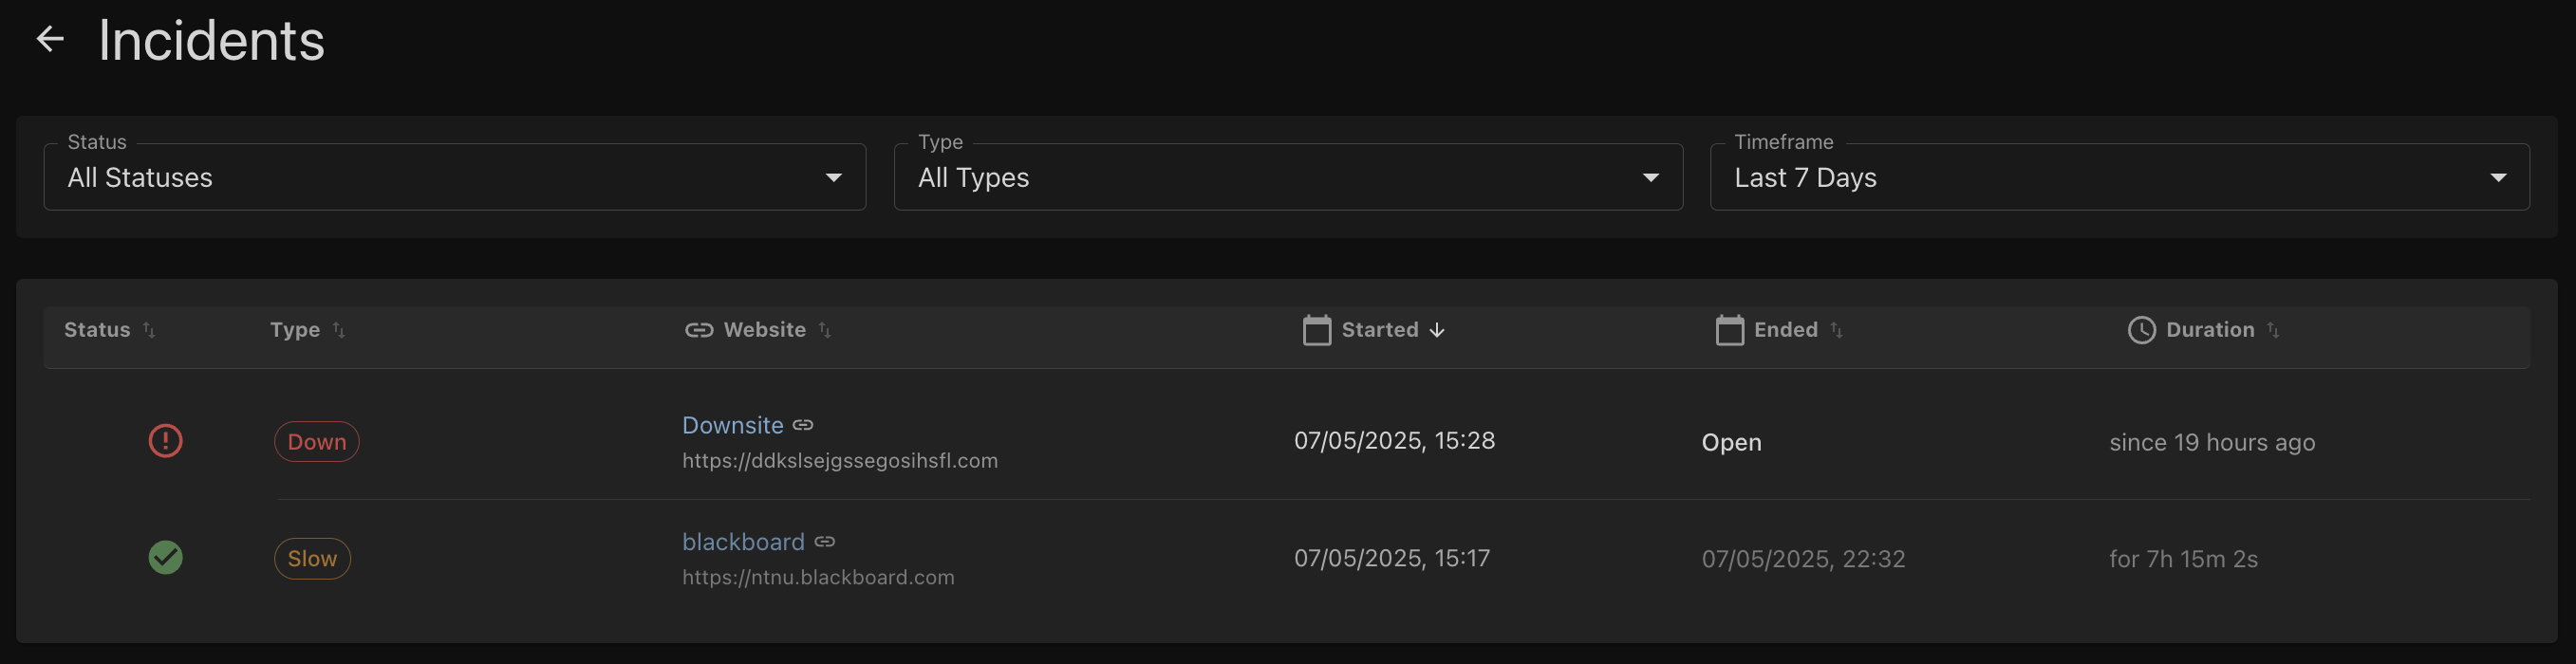
\includegraphics[width=1\textwidth]{figures/IncidentList.png}
\caption{Incident list visualisation in the monitoring dashboard}
\label{fig:incident_list}
\end{figure}



The Website Details page was view (Figure~\ref{fig:website_details_results}) was developed to provide users with tools for deeper investigation of website issues and status. It features performance graphs, status banners, and a timeline of incidents. These elements were incorporated in response to participant requests for more contextual data  The design applied Norman’s principles of visibility and feedback, offering users options such as selectable time frames for charts (1h, 24h, 7d, 30d, 1y), access to incident history, and recent check details. This fulfilled F8 (per-website historical data) and partially addressed F15 (graph labels). A persistent navigation bar at the top provides ongoing visibility of the overall status of all monitored websites.


\begin{figure}[H]
    \centering
    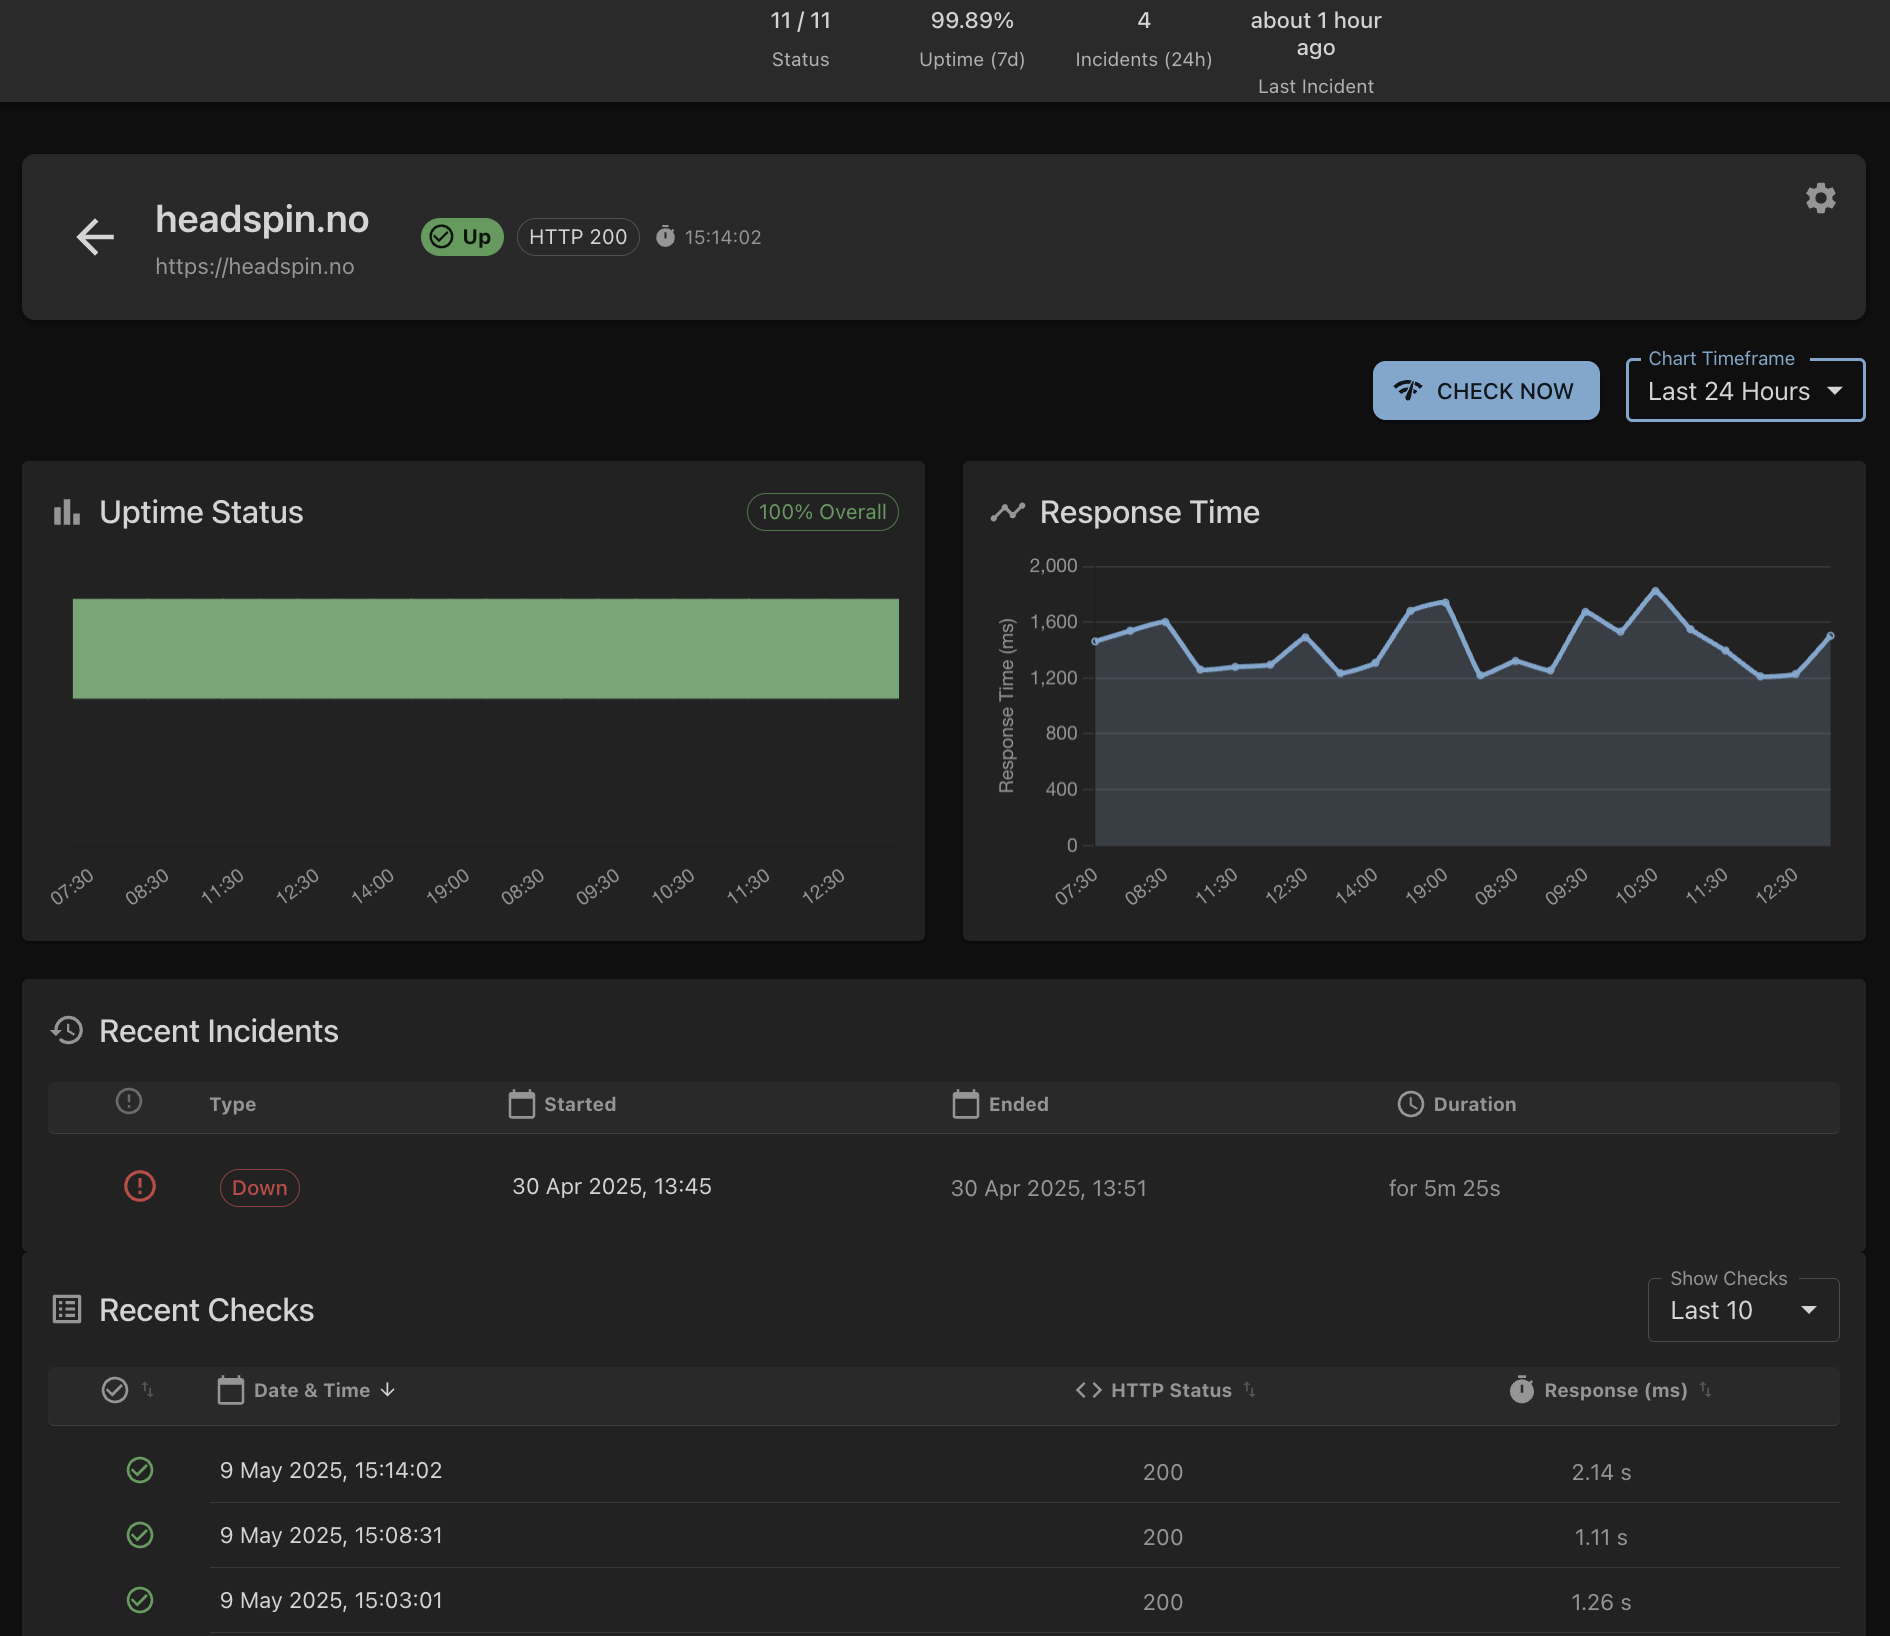
\includegraphics[width=1\linewidth]{figures/MVP-dashboard/MVP-websitedetails_full.png}
    \caption{Website Details}
    \label{fig:website_details_results}
\end{figure}

Theam toogle flyttet til user settings page

Back button på alle subpages (krav XX)

Historical 24 timer opp eller ned på hvert kort

Add website card on dashboard

Focus mode til tv mode

Fix status banner for å redusere vertikal space, søk, tv og filter flyttet inn i banner

Hover tooltip på graf

\subsubsection{Final Product Status}
The final version of the application therefore includes the existing navbar as well as a seperate card on the dashboard for navigating to the add website page. The status banner, search bar and filtering option was compacted into a single card using less vertical space, adhering to P1's feedback. In a attempt to improve the intuitiveness of the navigation back to the main dashboard page, a back button was added to  every subpage. Figure~\ref{header_websitedetails} shows an example of the back button on the website details page.
These changes complete the navigation refinements identified in feedback from user test 1 and 2.

The final version includes sparkline graphs on each website card (Figure~\ref{fig:websitecard_comparison}) and a revised Website Details page (Figures~\ref{fig:website_details_results}) with selectable timeframes: 1h, 24h, 7d, 30d, and 1y.  
An incident log is also available for contextual data.  
However, the main dashboard graph still lacked a title and legend at project hand-off (Table~\ref{tab:req_incomplete}, F-15).

Figure~\ref{fig:websitecard_comparison} illustrates the final card colours, and Figure~\ref{fig:website_details_results} shows the updated chart and status banners in the final version of the application.

Based on the feedback from user test 2 there was an attempt to solve some of the issues encountered. To start the thresholds were altered for the bar-chart on the Website Details page, indicating uptime. This was to make sure any actual downtime was caught and displayed. Both on the Website Details page but also on the new sparkline added to every card, displaying this same data below the graph, as seen in Figure~\ref{fig:wesitecard_final}.  

\begin{figure}
    \centering
    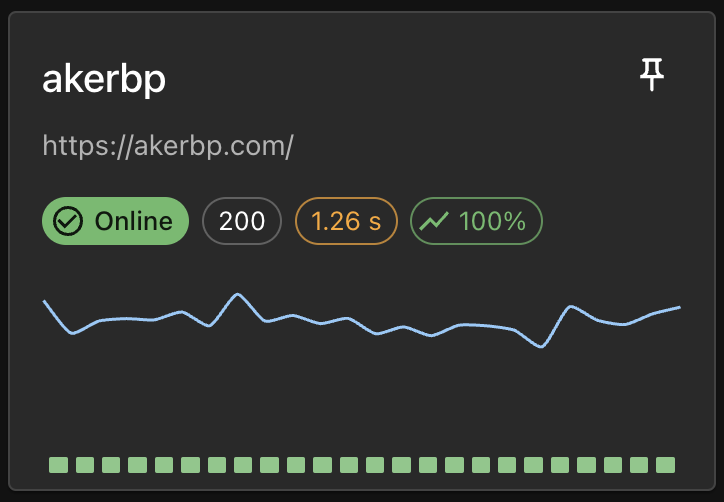
\includegraphics[width=0.75\linewidth]{figures/websiteCard.png}
    \caption{Website Card displaying current status, status-code, response time for last check, uptime, response time graph and sparkline for uptime}
    \label{fig:websitecard_final}
\end{figure}


tooltip on graph cards
fix vertical space status bar








\subsection{Quantitative Usability Evaluation (SUS Scores)}
\label{subsec:quant_sus}
After user test 2, all three participants completed the \acrshort{sus} form immediately after finishing their tasks, and before any debriefing took place. Their individual scores are shown in Table~\ref{tab:sus-scores}.

The following table shows the score of each participant scored according to the calculation guide from 

\begin{table}[H]
\centering
\begin{tabular}{@{}lccccccccccc@{}}
\toprule
\textbf{Participant} & \textbf{1} & \textbf{2} & \textbf{3} & \textbf{4} & \textbf{5} & \textbf{6} & \textbf{7} & \textbf{8} & \textbf{9} & \textbf{10} & \textbf{SUS} \\
\midrule
User 1 & 4 & 2 & 4 & 1 & 4 & 2 & 4 & 2 & 4 & 2 & 77.5 \\
User 2 & 4 & 2 & 4 & 2 & 4 & 1 & 5 & 1 & 4 & 1 & 85.0 \\
User 3 & 5 & 1 & 5 & 1 & 4 & 2 & 5 & 2 & 5 & 1 & 92.5 \\
\midrule
\textbf{Mean} &  &  &  &  &  &  &  &  &  &  & \textbf{85.0} \\
\bottomrule
\end{tabular}
\caption{Individual \acrshort{sus} item ratings and overall scores}
\label{tab:sus-scores}
\end{table}


The resulting mean \acrshort{sus} score of \textbf{85.0} places the MVP of the dashboard well above the standard industry benchmark of 68, which is commonly interpreted as the threshold for acceptable usability \autocite{MeasuringSUS2011}. According to SUS benchmark data~\autocite{Bangor2009}, a score of 85 falls into the 95–97\textsuperscript{th} percentile, corresponding to a “B” grade and indicating excellent usability. This score was recorded after iterative design changes described in Section~\ref{sec:rq1}.

\begin{figure}[H]
    \centering
    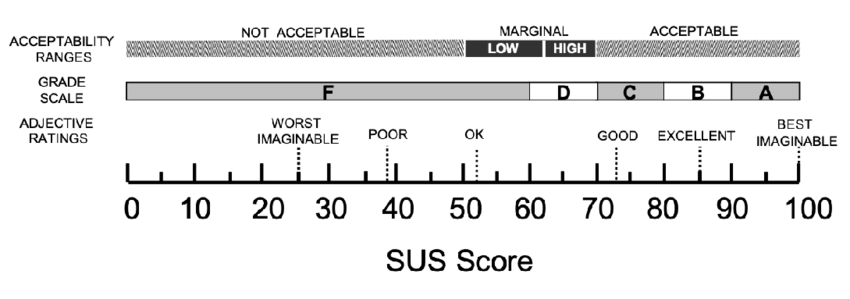
\includegraphics[width=0.8\textwidth]{figures/Grade-rankings-of-SUS-scores-from-An-Empirical-Evaluation-of-the-System-Usability.png}
    \caption{SUS Grade Rankings (adapted from \cite{Bangor2009})}
    \label{fig:sus_scores}
\end{figure}

\subsection{Final Application Design Features}
\label{subsec:final_app_design}

Design refinements, implemented in response to user feedback (summarised in Tables~\ref{tab:prototype-issues} and \ref{tab:mvp-issues}), were informed by design theories discussed in Chapter~\ref{ch:theory} (e.g., Nielsen’s heuristics, Norman’s interaction design principles, and Few’s dashboard guidelines). The resulting interface incorporated features such as dynamic ordering of dashboard cards, status indicators, and colour-coding, with the design goal of balancing information density and clarity.

\subsubsection{Dashboard Page Design}
The main dashboard (Figure~\ref{fig:main_dashboard}) was designed applying Few’s simplicity principle and Nielsen’s aesthetic and minimalist heuristic. Information presentation includes dynamic component ordering based on website status, iconography, and colour-based status indicators. Gestalt principles, including proximity, enclosure, and similarity, were applied to the layout of elements (as shown in Figure~\ref{fig:main_dashboard}), with the intention of improving visual organization and structure.

\begin{figure}[H]
    \centering
    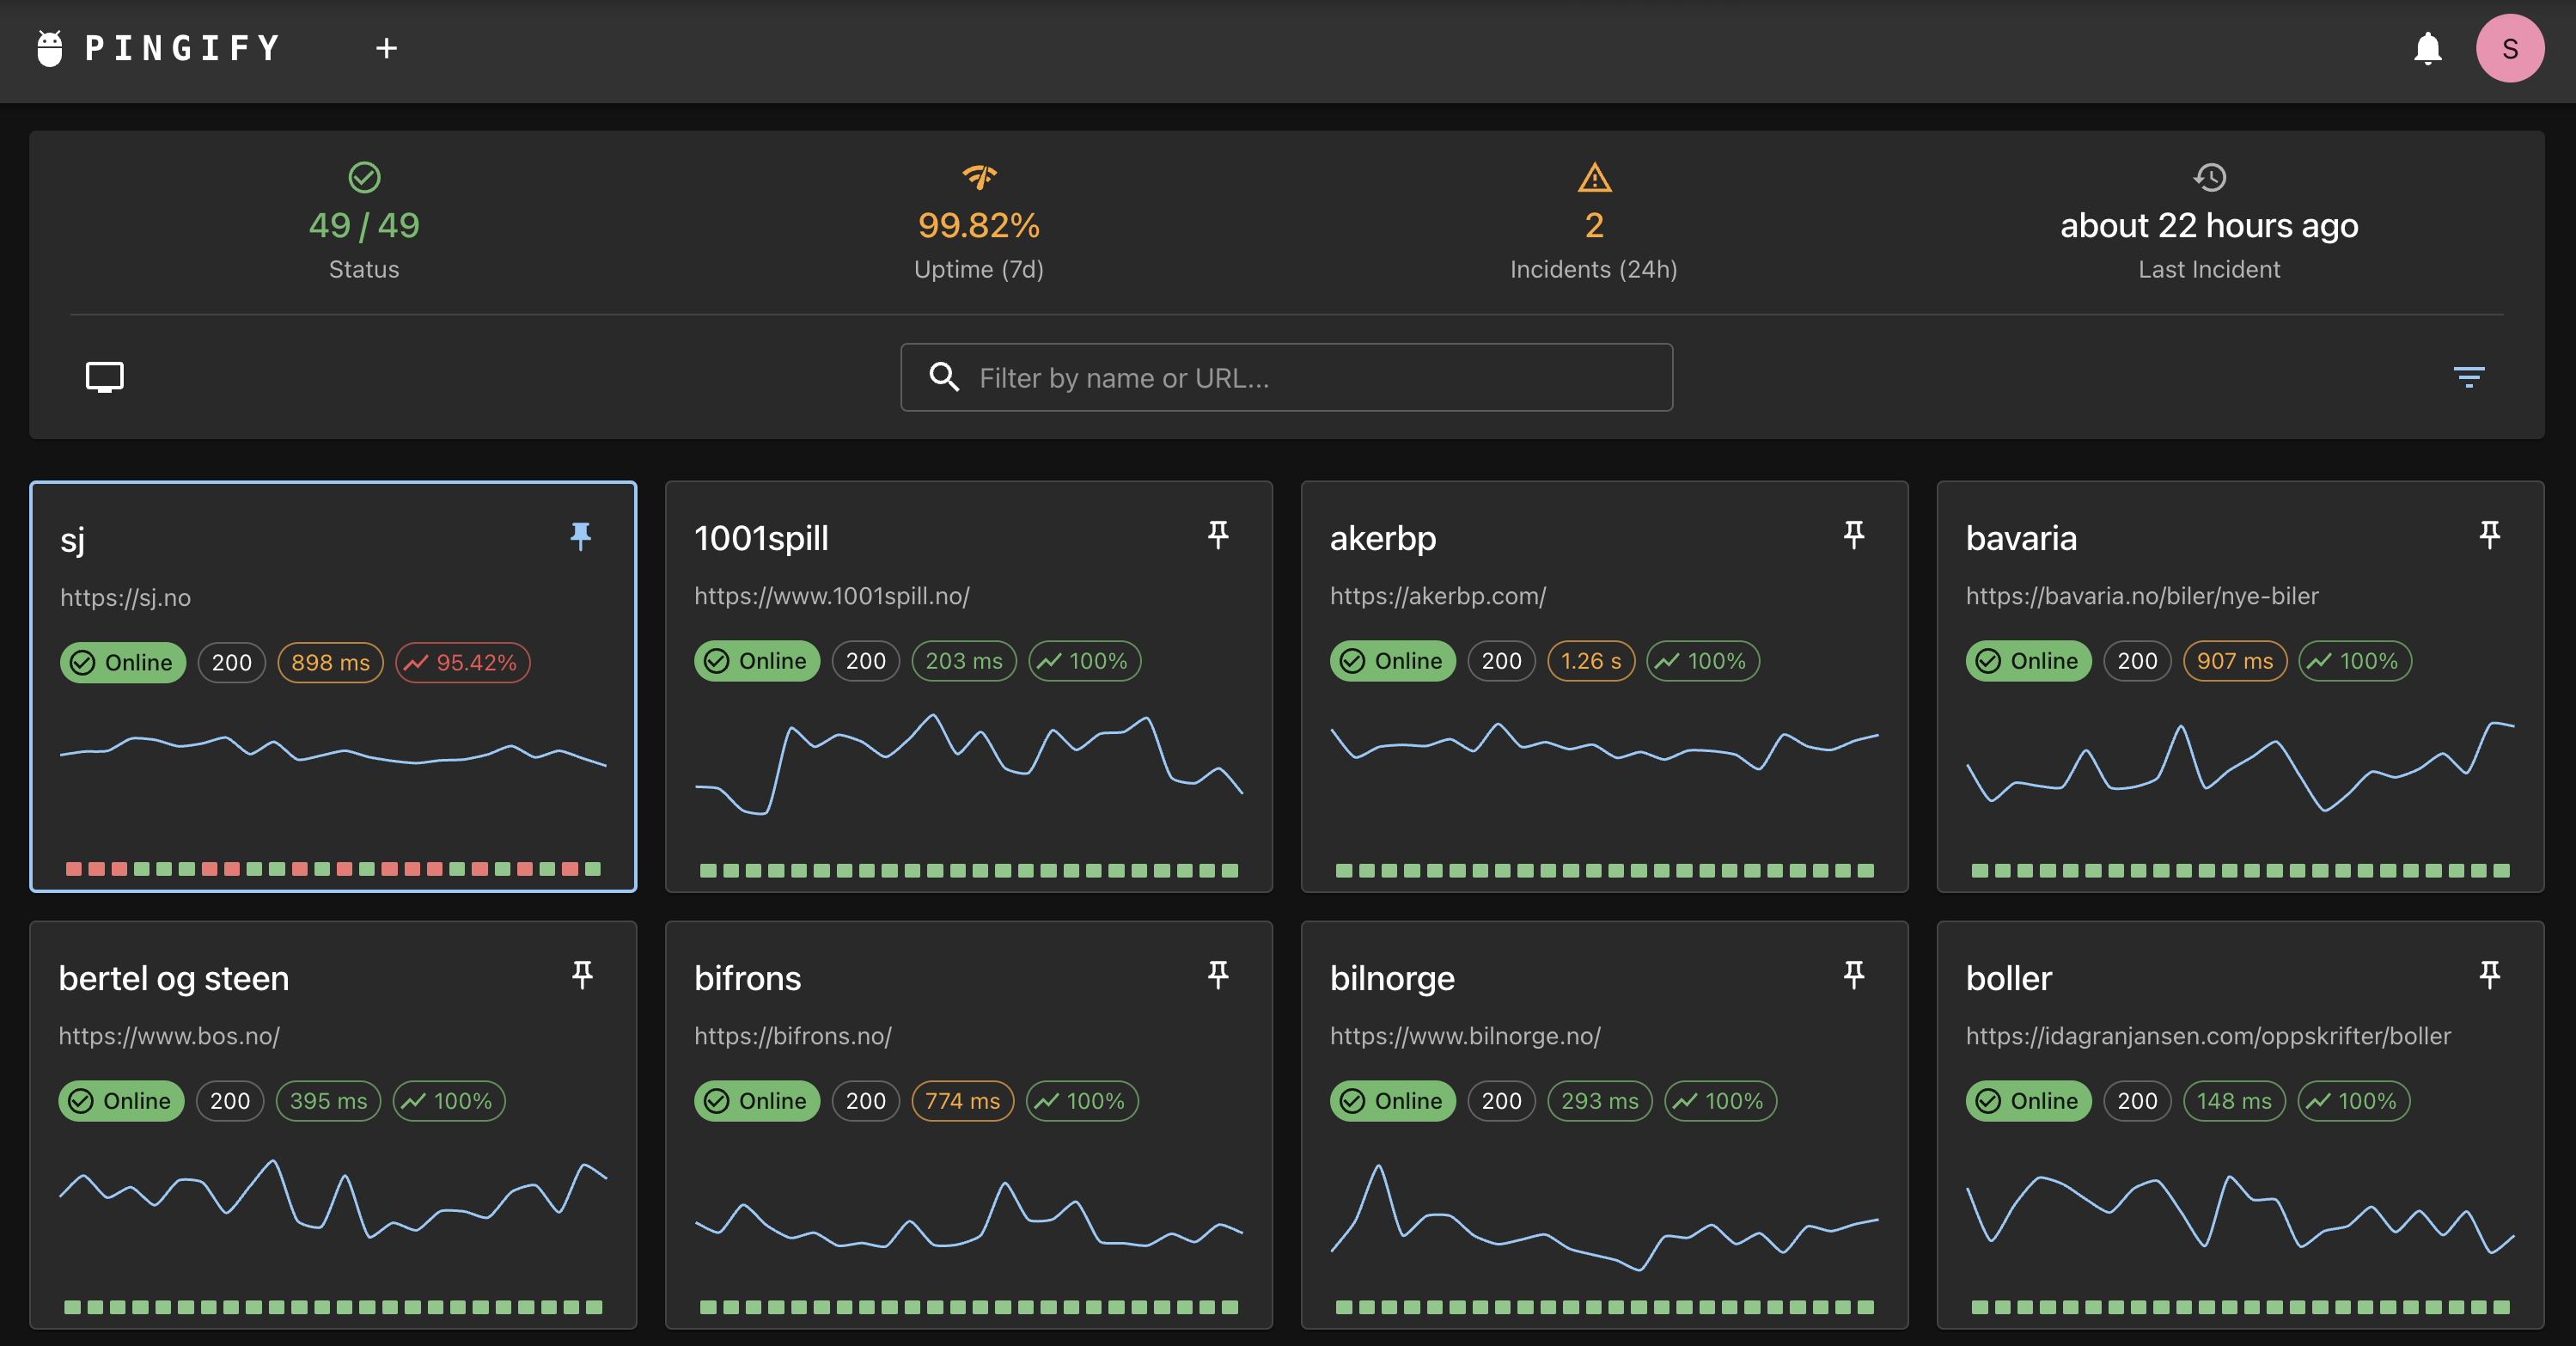
\includegraphics[width=1\linewidth]{figures/main_dashboard.png}
    \caption{Main Dashboard with Pinned Website}
    \label{fig:main_dashboard}
\end{figure}

\subsubsection{Website Card Design}
The Website Card (Figure~\ref{fig:websitecard_comparison}) displays the status of a website using real-time indicators. In response to feedback regarding insufficient detail from user test 1, (Table~\ref{tab:prototype-issues}), the design was updated to include additional data points. The visual styling aimed for clarity and consistency, aligning with Norman’s emphasis on usability and Nielsen’s “Consistency and Standards” heuristic~\autocite{Nielsen1994}, with the design objective of minimizing cognitive load.

\begin{figure}[H]
    \centering
    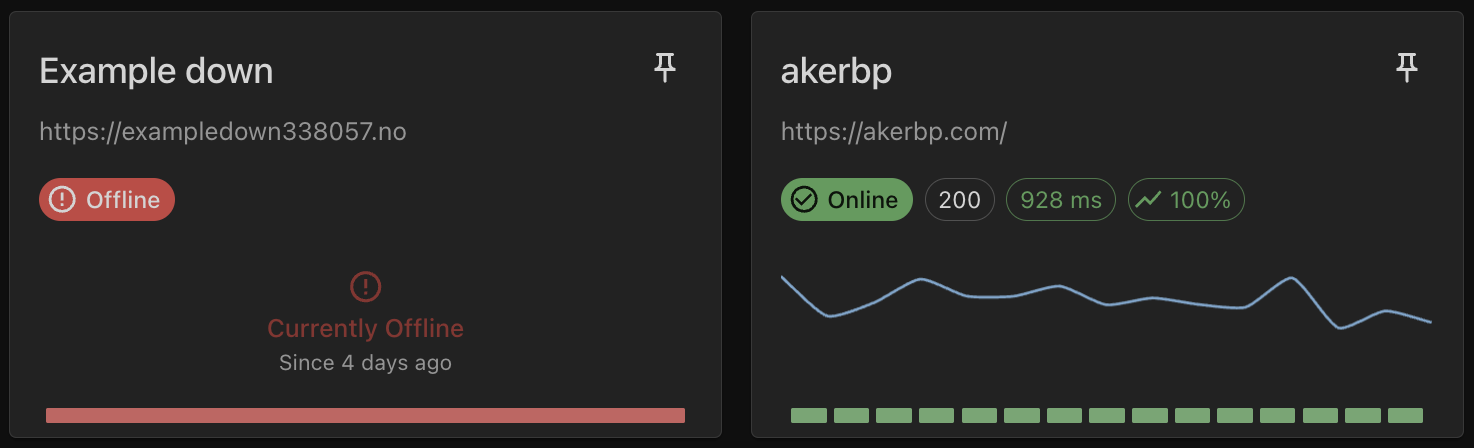
\includegraphics[width=1\linewidth]{figures/final_application/Final_card_comparison.png}
    \caption{Two Website Cards: One offline and one online}
    \label{fig:websitecard_comparison}
\end{figure}

\subsubsection{
\subsubsection{Key Design Changes}

The dashboard design evolved through iterative user testing, with changes made in response to specific usability issues raised during evaluations (summarized in Tables~\ref{tab:prototype-issues} and \ref{tab:mvp-issues}). These modifications also incorporated guidance from design principles outlined in Chapter~\ref{ch:theory}. Four key examples of these design changes are detailed below.

\paragraph{Navigation Bar}
\label{par:navbar_result}
Following feedback from user test 1 where participants expressed confusion over the original hamburger-style side menu (Table~\ref{tab:prototype-issues}), this element was removed. A persistent top navigation bar was implemented (Figure~\ref{fig:navbar}).

The redesigned navbar includes a home button (logo + title), a labeled button for adding websites (with tooltip), an alert indicator with a numeric badge, and a profile dropdown for user settings. This configuration was intended to make high-frequency actions immediately visible and accessible, aligning with Norman’s principles of affordance and visibility \parencite{sharp-2019}.

\begin{figure}[H]
    \centering
    
\includegraphics[width=1\linewidth]{figures/navbar.png}
    \caption{Navbar with changes made}
    \label{fig:navbar}
\end{figure}

\begin{figure}[H]
    \centering
    
\includegraphics[width=1\linewidth]{figures/navbar-status.png}
    \caption{Navbar while away from dashboard}
    \label{fig:navbar_status}
\end{figure}

To address discoverability, the "Add Website" function was also provided as a dedicated card component in the main dashboard grid (Figure~\ref{fig:addwebsitecard}). This design choice aligns with universal design principles by offering multiple access points for this critical task.

\begin{figure}[H]
    \centering
    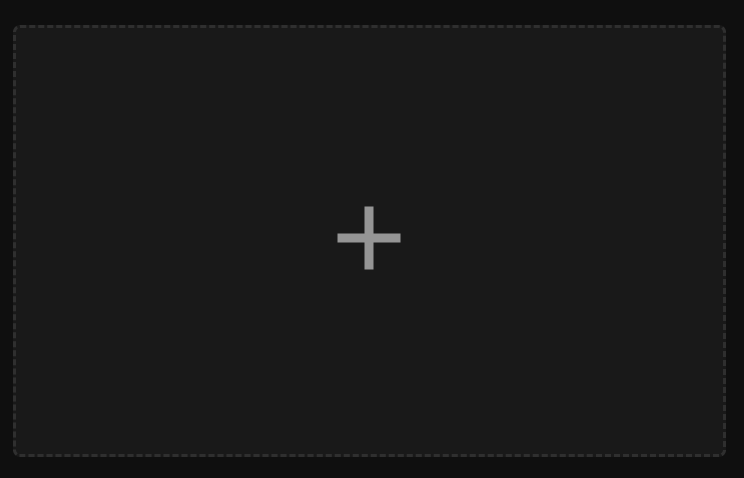
\includegraphics[width=0.5\linewidth]{figures/addwebsitecard.png}
    \caption{Add Website Card}
    \label{fig:addwebsitecard}
\end{figure}

\paragraph{Filtering and Pinning}
User test 1 feedback also indicated confusion regarding the placement of filtering options, originally in the sidebar (Table~\ref{tab:prototype-issues}). The filtering controls were subsequently relocated above the website cards on the right-hand side (Figure~\ref{fig:statusbar}). This decision considered conventional UI patterns and learned user behavior, as described by Norman \parencite{sharp-2019}.

The revised placement aimed to align with Few’s emphasis on contextual clarity  \parencite{FewDashboard}, to make filtering tools readily available without cluttering the interface.

The card-sorting logic was also refined to order content dynamically: pinned cards appear first, followed by websites with a 'down' status, then alphabetically ordered cards. This prioritization strategy was designed to improve at-a-glance interpretability with critical value exceptions and reflects Nielsen's heuristic of visibility of system status \parencite{Nielsen1994}. 

\begin{figure}[H]
    \centering
    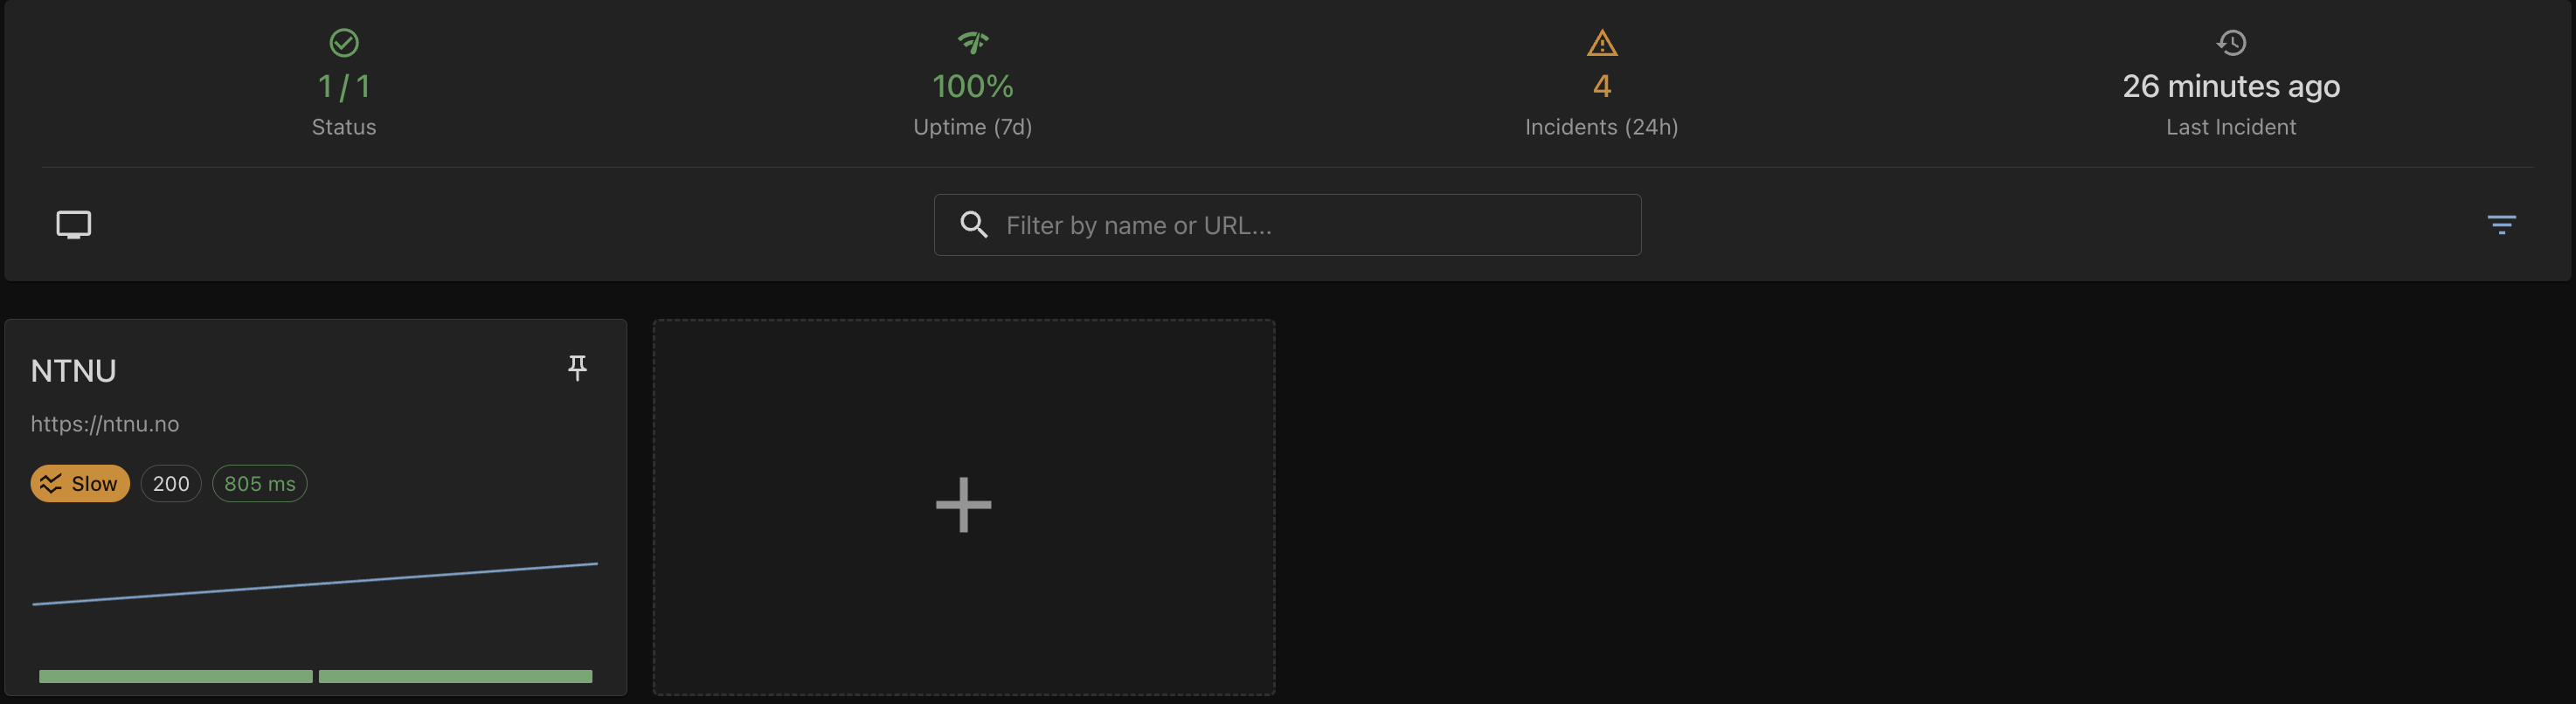
\includegraphics[width=1\linewidth]{figures/statusbar.png}
    \caption{Status Bar with TV-mode, Searchbar and Filtering}
    \label{fig:statusbar}
\end{figure}

\paragraph{TV-Mode}
TV-mode was developed in response to stakeholder and user feedback indicating that the dashboard would often be used passively on large screens. The feature, originally labeled “Focus-mode,” was renamed and its design was revised following feedback from user test 2.

As shown in Figure~\ref{fig:tv-mode}, TV-mode activates a fullscreen display which hides both the navbar and filter bar, thereby prioritizing the display of status cards.  These changes were informed by Few's principle of simplicity and single-screen visibility and Nielsen's heuristic of aesthetic and minimalistic design by reducing interface complexity. The icon and tooltip for TV-mode were redesigned after user test 2, influenced by Norman's principles of visibility, affordance and feedback. 

These changes were informed by Norman’s guidelines on intuitive feedback and mapping, and also aimed to align with Few’s emphasis on clarity for monitoring key metrics with minimal interface distraction.

\begin{figure}[H]
    \centering
    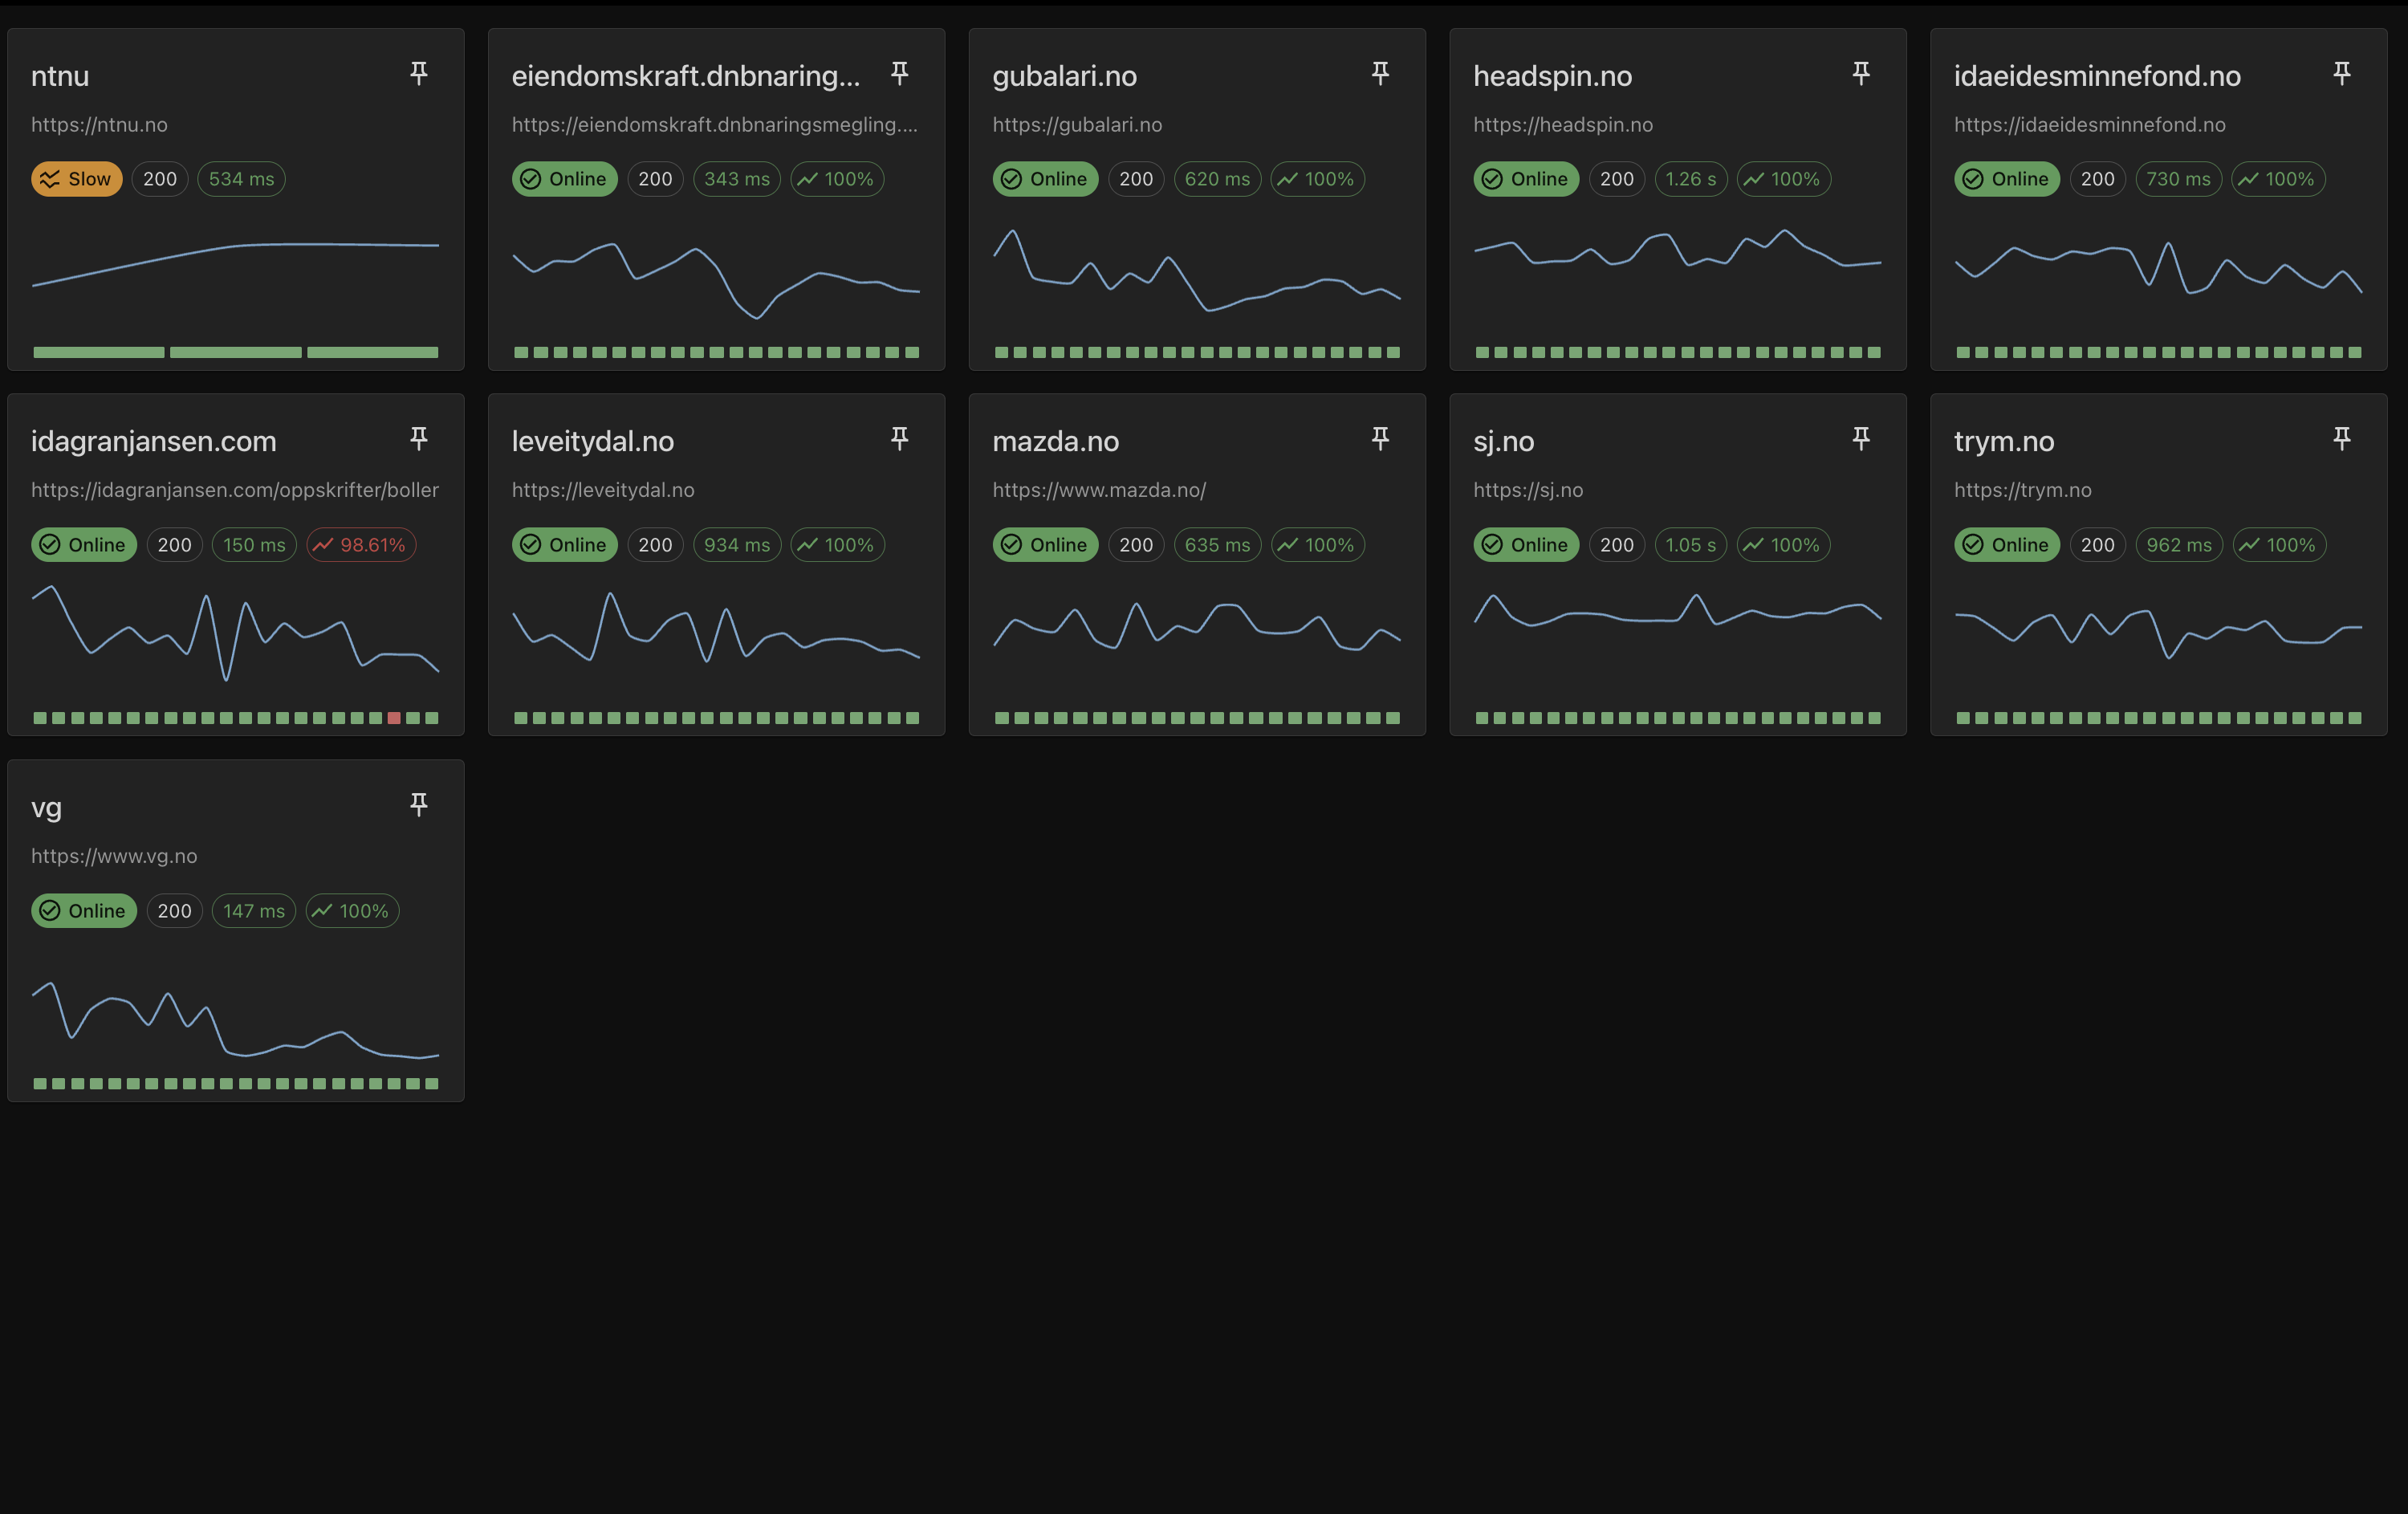
\includegraphics[width=0.75\linewidth]{figures/tv-mode.png}
    \caption{TV-Mode}
    \label{fig:tv-mode}
\end{figure}


\paragraph{Back-button in Details View}
The need for an explicit return path from the website details page to the dashboard was identified in user test 2. Consequently, the final application includes a dedicated back-button in the header of the website details page (Figure~\ref{fig:header_websitedetails}).

This addition was intended to provide users with greater control and freedom, aligning with a core heuristic from Nielsen \parencite{nielsen1994}, and was also a component in establishing navigational consistency. The design aimed to reduce reliance on browser controls for this action.

\begin{figure}[H]
    \centering
    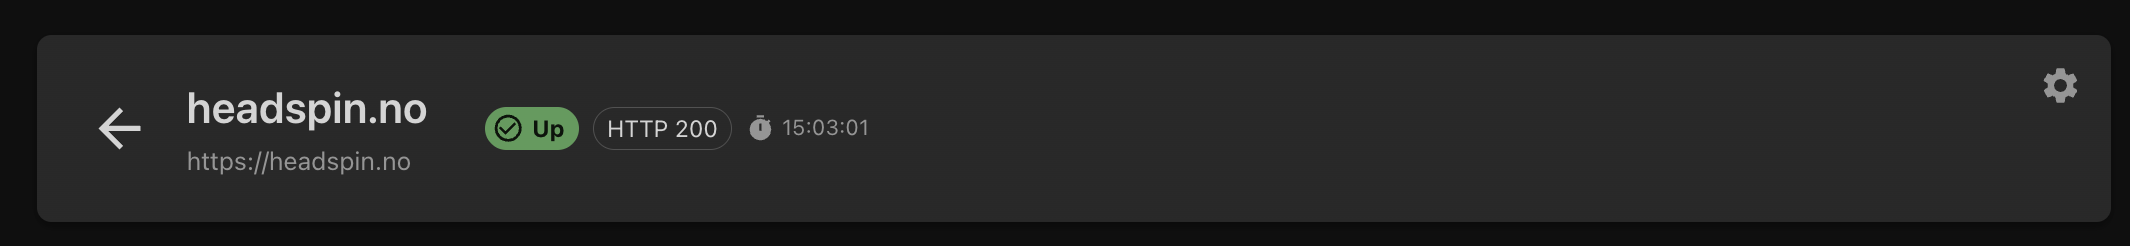
\includegraphics[width=1\linewidth]{figures/header_websiteDetails.png}
    \caption{Website Details Header with back-button, status indicators, and cogwheel for settings}
    \label{fig:header_websitedetails}
\end{figure}


%%%%%Her må vi vise hvordan kravene er blitt oppfylt med bilder fra dashboardet og linke til spesifikk krav (se incident list lengre ned)
\subsection{Iterative Development and Functionality Enhancements}
\label{sec:rq2}
This section addresses the second research question by detailing how the iterative development process, incorporating multiple rounds of feedback and requirement refinement, led to enhanced functionality and better user adaptation.



\subsection{Functional Enhancements and User Adaptation}
Several new features and refinements were implemented in direct response to feedback across development phases:

\begin{itemize}
    \item \textbf{Filtering and Sorting} (F7): Added after user test 1 to improve content navigation.
    \item \textbf{Configurable Alert Thresholds} (F10): Implemented post-MVP testing to give users control over performance sensitivity.
    \item \textbf{Incident System} (F11): Introduced to highlight and contextualise recurring or critical website issues.
    \item \textbf{User Authentication} (F5): Implemented using JWTs to support personalised dashboards.
    \item \textbf{Improved Navigation and Visual Hierarchies}: Based on feedback that sidebar menus and iconography were unintuitive or cluttered.
\end{itemize}

These changes were introduced between User Test 1 and the hand-off build.

\subsection{System Implementation Outcomes}
\label{sec:sys_implement_outcomes_results}
The developed dashboard system incorporated several key technical components. This section describes these components as they were implemented in the final version of the application.

\subsubsection{System Architecture and Sitemap}
The dashboard was implemented with a modular, multi-page structure, designed for navigation between core features including the main dashboard, website details, and incident tracking. This structure was refined as new functionality was added during iterative development. The final sitemap, illustrating the application's structure and page relationships, is presented in Figure~\ref{fig:sitemap_final}.

\begin{figure}[H]
\centering
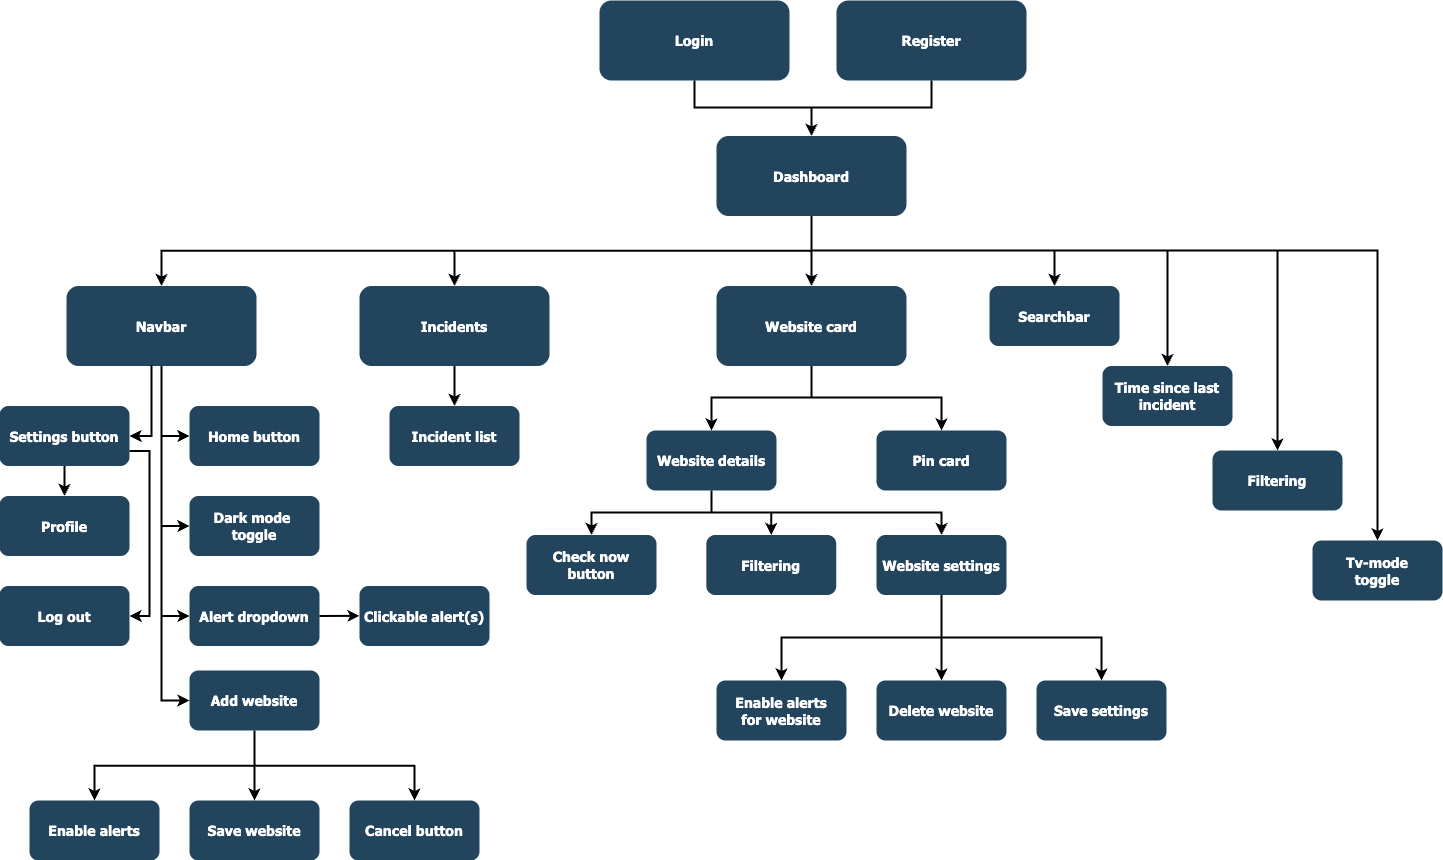
\includegraphics[width=\textwidth]{figures/diagrams/sitemap-final.png}
\caption{Final sitemap of the application structure and page relationships}
\label{fig:sitemap_final}
\end{figure}



\subsubsection{Incident Tracking System}
In response to feedback from user testing (Table~\ref{tab:mvp-issues}), an incident tracking system was implemented. This system allows dashboard users to track and visualize recurring issues for the websites they monitor. Incidents were generated based on consecutive monitoring failures and were displayed in both the main dashboard view and the website details view (Figure~\ref{fig:incident_list}).

\begin{figure}[H]
\centering
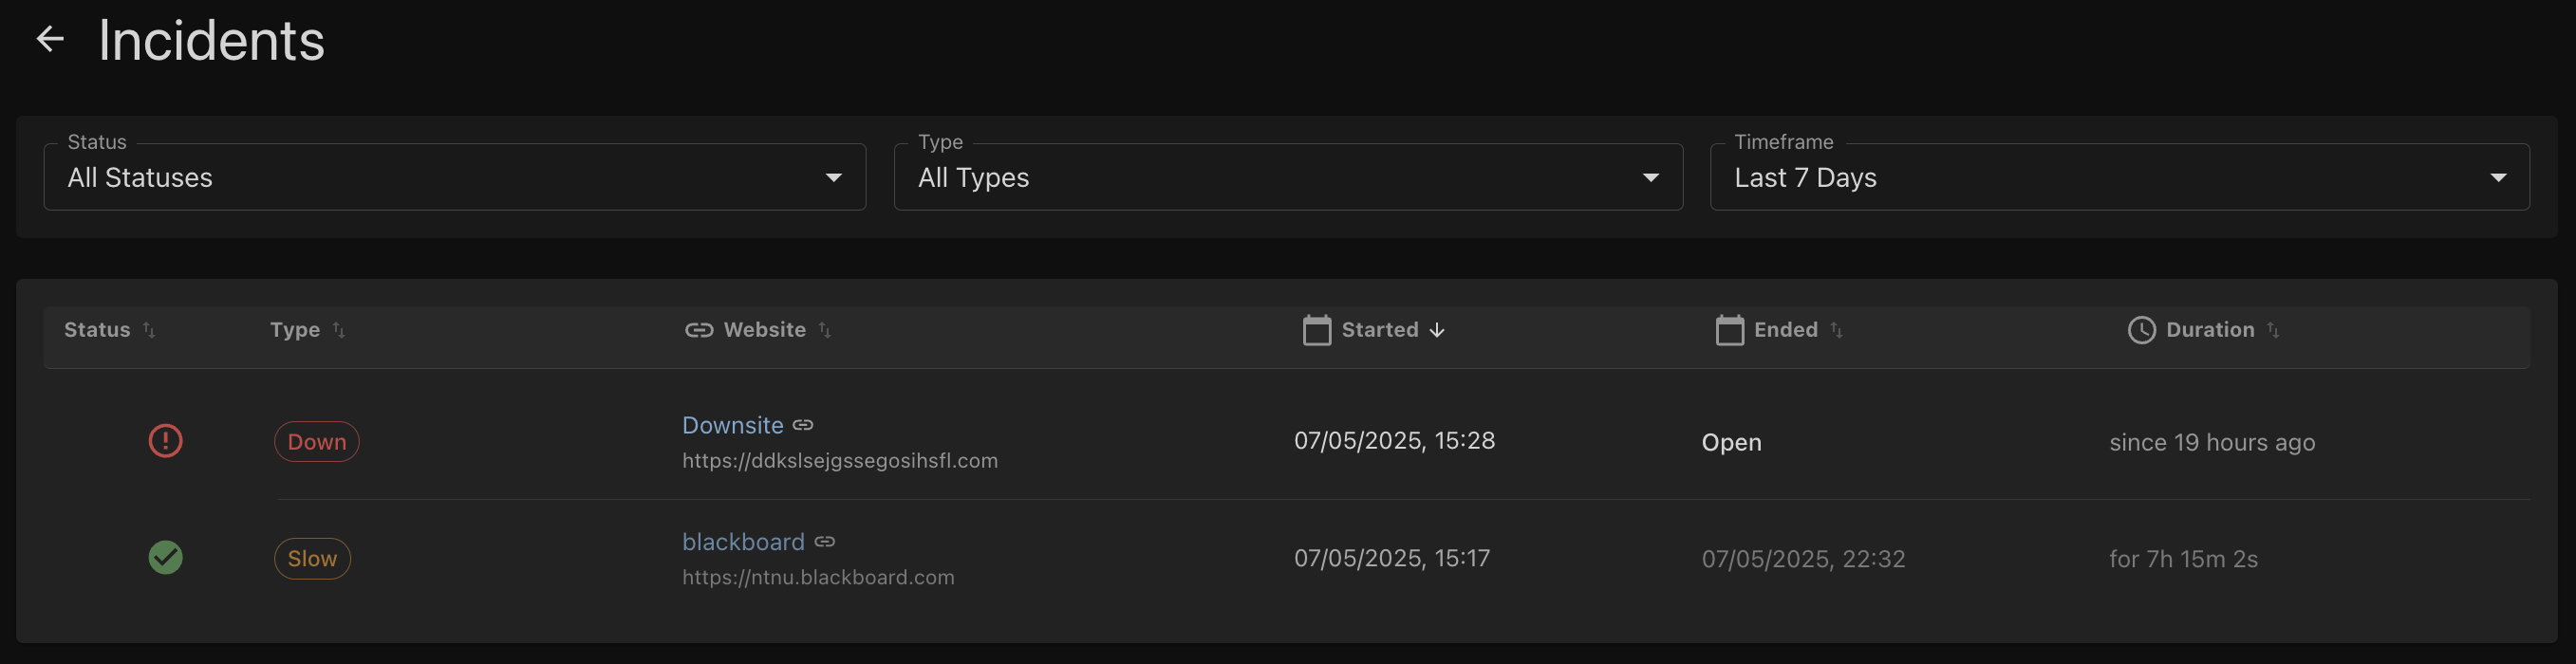
\includegraphics[width=1\textwidth]{figures/IncidentList.png}
\caption{Incident list visualisation in the monitoring dashboard}
\label{fig:incident_list}
\end{figure}



\subsection{Universal Design}
\label{sec:universal_design}

Several features were implemented to support universal design objectives, with the aim of improving accessibility and usability across a broad range of users and devices. These features contribute to the partial fulfilment of requirement NF3 (Table~\ref{tab:req_incomplete}), which relates to universal usability and responsive design.

\begin{itemize}
    \item \textbf{Colourblind mode}: An optional colourblind mode was added to improve visual accessibility. This mode adjusts the default colour scheme to enhance contrast and distinguishability for users with colour vision deficiencies. Examples of the modified interface are included in Appendix~\ref{app:colourblind_mode}.

    \item \textbf{Keyboard accessibility}: The dashboard supports navigation and interaction using only the keyboard. All form elements, buttons, and navigation components are operable using standard keys such as \texttt{Tab}, \texttt{Enter}, and \texttt{Escape}. Focus indicators and consistent tab order were maintained using accessible UI components.

    \item \textbf{Responsive design}: The layout and components of the dashboard are designed to adapt to various screen sizes and resolutions, including mobile phones, tablets, and widescreen monitors. Content remains readable and interactive across breakpoints, supporting use on different devices without requiring interface adjustments.
\end{itemize}

Some accessibility aspects, such as full screen reader support and contrast testing for all visual states, were outside the project scope and are candidates for future work.



\subsection{Requirement Fulfilment Overview}
\label{subsec:req_final}

To assess whether the system met its intended functional and quality goals, this section reviews the extent to which the defined requirements were fulfilled. A total of eighteen requirements—twelve functional (F) and six non-functional (NF)—were tracked from the initial brief to the final release (see \autoref{app:req_from_brief}–\autoref{app:req_mvp_user_test}).

To support clarity and post-project analysis, the requirements are grouped below into (i) those fully implemented in the delivered system and (ii) those partially fulfilled or deferred for future work.

\begin{table}[H]
\centering
\begin{tabular}{|l|p{0.60\linewidth}|c|}
\hline
\textbf{Req.\ ID} & \textbf{Requirement (functional \& non-functional)} & \textbf{Priority}\\ \hline
F.1  & User can add, edit and delete monitored websites via the user interface.& High   \\ \hline
F.2  & User can set custom check intervals per website.& High   \\ \hline
F.3  & Display status, response time, and uptime history for each website on its dashboard card.& High   \\ \hline
F.5& Trigger alerts and notifications via e-mail or sms& Medium \\ \hline
F.6& Implement user authentication with personalised dashboards.& Medium \\ \hline

F.7  & Add functionality for filtering and sorting of website cards.& Medium \\ \hline
F.8  & Implement per-website overivew of historical data& High   \\ \hline
F.9  & Let users pin websites to the top of the dashboard.& Medium \\ \hline
F.10 & User-configurable alert thresholds for performance.                      & Medium \\ \hline
F.11 & Incident tracking system with incident list.                             & Medium \\ \hline
F.12 & Users can click on incident on graph to jump to related check.& Medium \\ \hline 
 F.13& Sparkline with status indication below response time chart on cards.&Medium \\\hline \hline
NF.1 & Monitoring of 50+ sites without noticeable delay.                        & High   \\ \hline
NF.2 & Real-time status updates with clear visual change indicators.            & High   \\ \hline
NF.5 & Card colours revised to reduce visual overload while preserving clarity. & High   \\ \hline
NF.6 & Dashboard data refreshes in near real-time.               & High   \\ \hline
\end{tabular}
\caption{Requirements fully implemented in the final system}
\label{tab:req_complete}
\end{table}

\begin{table}[H]
\centering
\begin{tabular}{|l|p{0.55\linewidth}|c|c|}
\hline
\textbf{Req.\ ID} & \textbf{Requirement} & \textbf{Priority} & \textbf{Status}\\ \hline
F.4  & Verify end-to-end page integrity beyond HTTP 200. & High & Unmet \\ \hline 
F.14 & Incident list and last incident buttons visible on status header.& Low&Unmet\\ \hline 
F.15 & Title and legend on card chart& low&Unmet\\\hline\hline \hline
NF.3 & Interface universally user-friendly and fully responsive. & High & Partial \\ \hline
NF.4 & Maintainable, fully documented code base. & Medium & Partial \\ \hline
\end{tabular}
\caption{Requirements partially implemented or deferred}
\label{tab:req_incomplete}
\end{table}

\paragraph{Coverage}
\begin{itemize}
    \item \textbf{Fully implemented:} 16 of 21 requirements ($\approx$76\%)—including 12 functional and 4 non-functional.
    \item \textbf{Partially implemented or unmet:} 5 of 21 requirements ($\approx$24\%)—deferred or incomplete.
\end{itemize}

\paragraph{Notes on partially implemented or unmet items}
\begin{itemize}
    \item \textbf{F\,4 — Page integrity checks:} Not implemented. Verifying end-to-end content beyond HTTP~200 was deprioritised due to technical complexity.
    \item \textbf{F\,14 — Incident header actions:} The incident list and shortcut buttons intended for the status header remain unimplemented.
    \item \textbf{F\,15 — Graph titles and legends:} Graphs for downtime and performance lack descriptive titles and legends at project hand-off.
    \item \textbf{NF\,3 — Responsive usability:} The interface is optimised for desktop and tablet; further testing and improvements are required for mobile and assistive technologies (e.g., screen readers).
    \item \textbf{NF\,4 — Maintainability:} The system includes inline documentation and a project README; however, a full developer guide and API documentation remain incomplete.
\end{itemize}

\paragraph{Project Outcome and Iterative Impact}
The final system fulfills approximately 76\% of all defined requirements, including all core monitoring, alerting, and dashboard functionality prioritised by Headspin. Iteratively developed features—such as filtering and pinning (F7, F9), configurable alerts (F10), and the incident tracking system (F11)—demonstrate how user and stakeholder feedback directly shaped the system. Partially fulfilled or unmet requirements reflect deliberate trade-offs made to deliver a stable and usable MVP. These outstanding items now serve as a clear foundation for future development, as discussed in Chapter~\ref{ch:discussion}.



\section{Summary of Key Findings}
This chapter has presented results structured around the two main research questions.

For RQ1 (design theories and usability), iterative application of design principles—particularly those by Few, Norman, and Nielsen—led to targeted interface improvements including revised colour schemes, enhanced visual hierarchy, and navigation refinements. These changes were guided by usability testing, and their impact is reflected in the recorded mean System Usability Scale (\acrshort{sus}) score of 85.0 for the MVP. This score places the dashboard within the 95th–97th percentile, indicating excellent usability (Figure~\ref{fig:sus_scores}).

For RQ2 (iterative development), the system evolved through successive rounds of feedback and requirement refinement. These iterations contributed to the introduction of key functionality such as filtering, configurable alerts, and incident tracking. The progression and final status of all tracked requirements are outlined in Tables~\ref{tab:req_evolution_table} and \ref{tab:req_fulfilment_matrix}, with 76\% fully implemented by project completion.

\section{Relation to Project Objectives}
The final system delivers core functionality for real-time website monitoring, user-specific dashboards, and automated incident tracking. It integrates visual and interaction design principles with technical features aligned to stakeholder priorities and the original problem statement.

While several advanced requirements remain partially or fully unmet, the delivered MVP forms a strong foundation for further development. The next chapter reflects on these findings, assesses their broader implications, and discusses limitations, trade-offs, and directions for future work.
